\documentclass[11pt,a4paper]{article}
\usepackage[T1]{fontenc}
\usepackage[utf8]{inputenc}
\usepackage{lmodern,microtype}
\usepackage[margin=25mm,headheight=15pt]{geometry}
\usepackage{amsmath,amssymb,amsthm,mathtools}
\usepackage{booktabs,longtable,tabularx,array}
\usepackage{xcolor,graphicx}
\usepackage{tikz}
\usetikzlibrary{arrows.meta,positioning,fit,calc}
\usepackage{enumitem,listings,fancyhdr,needspace,xurl}
\usepackage[colorlinks=true,linkcolor=blue!45!black,citecolor=green!35!black,urlcolor=blue!50!black]{hyperref}
\usepackage{bookmark}

\definecolor{ink}{HTML}{172B3A}
\definecolor{accent}{HTML}{235F7B}
\definecolor{pale}{HTML}{F1F5F7}
\definecolor{rulecol}{HTML}{BDCCD5}

\newcommand{\code}[1]{\texttt{\detokenize{#1}}}
\newcommand{\Lean}{Lean~4}
\newcommand{\E}{\mathcal{E}}
\newcommand{\G}{\mathcal{G}}
\newcommand{\Pol}{\Pi}
\newcommand{\Bud}{\mathcal{B}}
\newcommand{\Obs}{\mathcal{X}}
\newcommand{\Comp}{\mathrm{Comp}}
\newcommand{\Beh}{\mathrm{Beh}}
\newcommand{\Sort}{\mathrm{Sort}}
\newcommand{\Prop}{\mathrm{Prop}}
\newcommand{\Nat}{\mathbb{N}}
\newcommand{\Pn}[1]{P#1}
\newcommand{\prov}[1]{\textsuperscript{\scriptsize[#1]}}
\newcolumntype{Y}{>{\raggedright\arraybackslash}X}
\newcolumntype{L}[1]{>{\raggedright\arraybackslash}p{#1}}

\setlist{nosep,leftmargin=1.6em}
\setlength{\parskip}{4pt}
\setlength{\parindent}{0pt}
\setcounter{tocdepth}{2}
\setcounter{secnumdepth}{3}
\emergencystretch=4em
\raggedbottom
\widowpenalty=10000
\clubpenalty=10000

\pagestyle{fancy}
\fancyhf{}
\fancyhead[L]{\small\color{ink}Leant2: unified architecture proposal}
\fancyhead[R]{\small Synthesis of nine design proposals}
\fancyfoot[C]{\thepage}
\renewcommand{\headrulewidth}{0.3pt}

\lstdefinelanguage{LeanSketch}{
  morekeywords={def,theorem,example,structure,inductive,where,match,with,fun,forall,let,in,by,exact,apply,intro,cases,induction,constructor,if,then,else,return,do,namespace,end,universe,termination_by,decreasing_by,noncomputable,partial,import,open,instance,class,abbrev,axiom,opaque,private,elab,syntax,macro,deriving},
  sensitive=true,morecomment=[l]{--},morecomment=[s]{/-}{-/},morestring=[b]"
}
\lstset{language=LeanSketch,basicstyle=\ttfamily\small,keywordstyle=\bfseries\color{accent},commentstyle=\itshape\color{black!55},backgroundcolor=\color{pale},frame=single,rulecolor=\color{rulecol},breaklines=true,columns=fullflexible,keepspaces=true,showstringspaces=false,aboveskip=8pt,belowskip=8pt,xleftmargin=3pt,xrightmargin=3pt}

\theoremstyle{definition}
\newtheorem{definition}{Definition}[section]
\newtheorem{invariant}[definition]{Invariant}
\newtheorem{decision}[definition]{Decision}
\theoremstyle{plain}
\newtheorem{proposition}[definition]{Proposition}
\newtheorem{theorem}[definition]{Theorem}
\theoremstyle{remark}
\newtheorem{remark}[definition]{Remark}

\tikzset{box/.style={draw=accent,rounded corners=2pt,fill=pale,align=center,inner sep=5pt,font=\small},
         flow/.style={-{Latex[length=2mm]},thick,draw=accent}}

\title{\textbf{Leant2: A Unified Architecture Proposal}\\[6pt]
\large Lean-native synthesis of programs and their contracts,\\
consolidated from nine independent design proposals}
\author{Prepared for Vladimir Reshetnikov}
\date{September 17, 2026}
\hypersetup{pdftitle={Leant2: A Unified Architecture Proposal},pdfauthor={Leant2 project},pdfsubject={Unified architecture and algorithm proposal for a Lean-native successor to Leant and Djex}}

\begin{document}
\maketitle

\begin{abstract}
Nine independently prepared design proposals for Leant2, a Lean-native successor to the Haskell synthesizers Leant and Djex, were written against the same repository snapshots and the same Lean~4.34.0 toolchain. They agree on more than they disagree. This document consolidates them into one proposal. Its architectural core is the consensus of all nine: exact Lean expressions as the only semantic authority; a transactional search whose unit of backtracking is a partial program together with \emph{all} of its unfinished obligations; recursion admitted only through typed schemas with explicit recursive-call capabilities; behavioral information with graded authority, where tests refute, proofs certify, and only proof-producing analyses may prune; and one acceptance gate that kernel-checks the exact program and the exact contract before anything is published. Where the proposals differ, this document selects the best-developed treatment and records its origin.

Two requirements come from the project owner rather than from the proposals. First, Leant2 has a single adaptive engine: no engine switches and, for now, no user-facing settings. Second, the minimal acceptance baseline is the existing Leant \code{:synth} golden corpus, thirty transcripts with 278 queries, read semantically: Leant2 must match or exceed every recorded outcome, but may return better candidates in a different order. Nothing here adds new experimental evidence; the evidence sections cite the nine packages and the sibling project Forge, whose kernel-checked certificate checkers and orchestration frontend Leant2 should reuse.
\end{abstract}

\vspace{4pt}
\textbf{Status.} This is a design specification. The nine source proposals each contain a small remotely compiled Lean prototype; collectively they demonstrate the continuation-backtracking core, dependent witness selection, dictionary identity, finite counterexample-guided synthesis, and hand-supplied certified recursion. They do not demonstrate automatic recursion discovery, library indexing, scheduling, or the acceptance gate. Section~\ref{sec:evidence} states exactly what has and has not been shown.

\clearpage
\tableofcontents
\clearpage

\section{Objective, baseline, and sources}\label{sec:scope}

\subsection{What Leant2 is}

Leant and Djex generate implementations for a subset of Lean type signatures, optionally under behavioral constraints. Both are implemented in Haskell, both search over a Haskell-shaped approximation of Lean types, and Djex must remain compatible with its Haskell frontend. Leant2 is the successor that removes all three limitations: it is implemented in Lean, it has only a Lean frontend, and it is designed for Lean types together with behavioral constraints. It cannot decide inhabitation of arbitrary Lean types, and no proposal claims that it can. The target is a large fraction of the types that occur in practice, with every positive answer checked by Lean's kernel.

Three constraints on this document come from the project owner and override anything in the nine source proposals.

\begin{decision}[Single adaptive engine]\label{dec:single-engine}
Leant2 has one engine. There are no engine switches of the kind Leant exposes (\code{synth-engine djinn | exference | both}), and no user-facing settings are implemented at first. Budgets, lane weights, verification windows, and candidate counts are internal parameters of an adaptive scheduler (Section~\ref{sec:scheduling}), derived from the query and from search progress, not from the user. Configuration may be added later behind the same engine, but no acceptance criterion in this document depends on it.
\end{decision}

\begin{decision}[Semantic baseline]\label{dec:baseline}
Leant2 must pass every \code{:synth} test in the Leant repository, read semantically: for each recorded query it must match or exceed the recorded outcome. It may return more candidates, better candidates, and candidates in a different order. Section~\ref{sec:baseline} makes this precise.
\end{decision}

\begin{decision}[Reuse of Forge]\label{dec:forge}
Forge is a sibling project with kernel-checked certificate checkers, an orchestration frontend with full rollback and proof-term auditing, and a written review of the Leant/Djex verification boundary. Leant2 may freely borrow Lean code and ideas from it, and this document does so explicitly (Section~\ref{sec:forge}).
\end{decision}

\subsection{How this document was produced}\label{sec:method}

The nine proposals are numbered \Pn{1} to \Pn{9} in the order of their directories under \code{docs/proposals/}. Each is a 32-to-45-page article with a small Lean~4.34.0 prototype checked remotely through the AXLE service, transcribed receipts, and helper scripts. All nine inspected the same Leant revision \code{6bf05ad} and one of two Djex revisions (\code{e8778f4}, the standalone head, or \code{e237e86}, the submodule pinned by Leant); three of them note that the two must not be conflated.

The consolidation rule is simple. An idea present in most proposals is adopted as core and stated once in its clearest form. Where proposals differ in the treatment of one subsystem, the best-developed version is adopted and the alternatives are recorded in Appendix~\ref{app:provenance}. Ideas are marked with their origin as \prov{\Pn{n}} on first use so that the more detailed discussion in the source can be consulted; a marker lists only the proposals that develop the idea most fully, not every proposal that mentions it. Nothing in this document is new evidence. Where the proposals' prototypes have shown something, Section~\ref{sec:evidence} says which one and how.

Names are unified as follows. What the proposals call the \emph{obligation graph}, \emph{goal forest}, \emph{hole graph}, or \emph{coupled continuation} is called the \emph{obligation graph} here. What they call \emph{recipes}, \emph{search plans}, \emph{construction plans}, or the \emph{control language} is called the \emph{search plan}. What they call \emph{acceptance}, \emph{admission}, \emph{publication}, \emph{finalization}, or the \emph{candidate gate} is called the \emph{acceptance gate}. Their result taxonomies, which range from five to nine constructors, are merged into the single result algebra of Section~\ref{sec:results}.

\subsection{The baseline: Leant's \code{:synth} corpus}\label{sec:baseline}

The Leant repository carries thirty golden-transcript fixtures \code{test/synth-*.txt}, each piped into \code{leant --plain} and diffed against \code{test/synth-*.golden} by \code{test/run-tests.sh}. Together they contain 278 \code{:synth} queries. Of these, 266 produce at least one displayed candidate, five produce the verdict ``provably uninhabited'', and seven are deliberate negative controls: three ``no term found within the search bounds'' under restricted provider settings, two ``none passed both Lean verification and the supplied assertion'', one assertion that fails type checking, and one assertion mentioning an unknown name. Twelve queries carry a behavioral assertion in the form \code{:synth f : T where P}. Appendix~\ref{app:corpus} tabulates the fixtures.

The transcripts also contain session declarations (\code{inductive}, \code{structure}, \code{class}, \code{instance}, \code{axiom}, \code{opaque}, \code{def}, \code{abbrev}, \code{universe}), \code{:reset}, and 170 \code{:set} lines that switch engines and adjust steps, windows, verification counts, classical mode, library use, and provider discovery. The recorded outputs include exact candidate spellings, ranking order, truncation notes, and engine-specific telemetry.

The goldens cannot be matched textually by a different engine, and Decision~\ref{dec:single-engine} removes the settings they exercise. The baseline is therefore defined on outcomes, not on text.

\begin{definition}[Baseline corpus]\label{def:corpus}
The baseline corpus is the set of \code{:synth} queries in \code{test/synth-*.txt} at Leant revision \code{6bf05ad}, each taken together with the session declarations that precede it in its transcript, and each labeled with the outcome recorded in the corresponding golden file. Every \code{:set} line is ignored. The recorded outcome of a query is one of: \emph{positive} (at least one displayed candidate), \emph{uninhabited} (``provably uninhabited''), \emph{bounded miss} (``no term found within the search bounds''), \emph{rejected} (candidates proposed, none passed), or \emph{preflight error} (assertion rejected before search).
\end{definition}

\begin{definition}[Baseline acceptance]\label{def:baseline}
Leant2 passes the baseline when, for every query in the baseline corpus, run under Leant2's default policy with no per-query configuration and within a fixed per-query wall-clock budget:
\begin{enumerate}
\item \textbf{Positive.} Leant2 returns at least one \emph{accepted} candidate: kernel-checked at the exact requested type in the exact session context and, for a \code{where} query, with a kernel-checked proof of the assertion for that exact candidate. The candidate need not be the recorded one, and the order of candidates is unconstrained.
\item \textbf{Uninhabited.} Leant2 returns a \emph{refutation} (a kernel-checked proof of $T \to \mathrm{False}$ in the session context) or a \emph{certified fragment non-derivability} (Section~\ref{sec:results}). For four of the five recorded cases a refutation exists and is preferred; the fifth, \code{forall p : Prop, p or not p}, is classically provable and must not be reported as refuted.
\item \textbf{Bounded miss, rejected.} Leant2 returns either an accepted candidate (this exceeds the recorded outcome and is allowed) or a qualified negative. It must not return an unaccepted candidate as a success.
\item \textbf{Preflight error.} Leant2 rejects the query before search with a diagnostic of the same category (ill-typed assertion; unknown name).
\end{enumerate}
The set of accepted candidates is a superset in strength of Leant's: any candidate Leant2 displays has passed the acceptance gate of Section~\ref{sec:acceptance}, which is stricter than Leant's re-elaboration.
\end{definition}

Three consequences follow. First, the five \code{synth-church-rankn}-style fixtures with 69 rank-N and Church-encoding queries are part of the baseline; they exercise nested polymorphic callbacks, universe-polymorphic families, strict-implicit binders, and seeded Church compositions, and are the hardest part of the corpus for a native engine that does not inherit Djex's rank-N machinery. Second, the \code{synth-library} fixture requires library composition (\code{List.map}, \code{List.foldr}, \code{List.flatten}, \code{List.replicate}) from the standard environment, so the provider index of Section~\ref{sec:library} is on the baseline path, not a later milestone. Third, the classical candidates in \code{synth-manual} (Peirce's law, double-negation elimination, and the like, produced with \code{synth-classical on}) count as positive outcomes; Leant2 must be able to offer \code{Classical.em}-based candidates, labeled as classical, when constructive search returns a certified fragment non-derivability (Section~\ref{sec:classical}).

The baseline is a floor. Leant's further suites also drive \code{:synth}: the Church behavior ledger (160 cells, 94 with historical acceptance), \code{test-recursive} (eight recursive-data behavioral scenarios with independent Lean replay), \code{test-behavioral} (bounded simplification and combined decision controls), and \code{test-context} (global class-projection discovery). These form the \emph{extended tier} of Section~\ref{sec:evaluation}: Leant2 should reach them after the baseline, and their historically accepted cells are regression targets, not gates for the first release.

\subsection{What the predecessors established}\label{sec:predecessors}

The proposals read the same sources and reach the same conclusions about them.

\textbf{Leant's representation boundary.} Leant elaborates queries in Lean and rechecks every candidate in Lean, but its search runs in Djex over a serialized fragment (\code{src/Leant/Synth/Fragment.hs}). The serializer retains structural connectives and selected polymorphic applications but treats term-indexed applications as opaque and describes recursion by bounded templates. This is the boundary Leant2 removes\prov{all}.

\textbf{Djex's two traditions.} Djinn is a checked propositional prover based on Dyckhoff's contraction-free calculus LJT; it terminates and can report that no derivation exists in its fragment. Exference is a ranked best-first search with class-evidence resolution and resource controls. Djex's shared infrastructure enforces source ownership, scoped evidence, and independent checking. Leant2 keeps those disciplines without the Haskell compatibility surface\prov{\Pn{6},\Pn{8}}.

\textbf{Behavioral assertions.} At the inspected revision, Leant checks a named assertion against each exact candidate by \code{decide}, then its negation, then bounded \code{simp} at both polarities; it distinguishes passed, falsified, and inconclusive, and never treats proof failure as a counterexample. Search produces type inhabitants first and filters afterwards. Every proposal moves the assertion into the search state so that it constrains witnesses before a candidate exists, while retaining the three-way distinction\prov{all}.

\textbf{The indexing gap.} Leant's current diagnostics locate the remaining integer-indexing failure in bounded composition: a function-valued fold and the integer case step are each found in isolation and missed in composition within the original limits. This motivates the demand-directed component reuse and carrier invention of Section~\ref{sec:library}. No proposal claims to have solved that fixture\prov{\Pn{1},\Pn{6},\Pn{7},\Pn{9}}.

\textbf{The earlier rewrite study.} The Leant repository's own rewrite analysis recommends Lean-hosted semantics, project-matched worker processes, exact source identities, and a kernel validation boundary; those are adopted. It also recommends a pure, neutral search representation with native metavariables confined to preparation and lowering. All nine proposals depart from that point: a neutral representation restricted enough to be easy to search recreates the loss of dependency information the successor is meant to remove. Leant2 searches over native, branch-local dependent constraints, and keeps a serializable plan only for replay, caching, and cross-process transfer (Section~\ref{sec:representations})\prov{\Pn{1},\Pn{6},\Pn{9}}.

\subsection{What to take from Forge}\label{sec:forge}

Forge \cite{forge} is a certificate-producing proof-planning layer above \code{grind}. It pins the same toolchain as the nine proposals, Lean~4.34.0 with Mathlib \code{1cf325a0}, and has reached a state none of the Leant2 prototypes has: compiled Lean with proved soundness theorems and a measured comparison. Four parts transfer directly.

\begin{enumerate}
\item \textbf{The orchestration frontend} (\code{lean/Forge/Frontend.lean}). The \code{forge} tactic runs a fixed list of workers, saves the full tactic state before each, restores it on any failure including resource limits, and on apparent success does not take the worker's word: it instantiates the proof term and rejects it if it contains \code{sorry}, mentions a free variable outside the goal's context, fails to type-check against the \emph{original} goal, or depends on an axiom outside the policy, computed with \code{collectAxioms} over the constants the term uses. It then emits a replay record. This is exactly the proof-service contract of Section~\ref{sec:proof-services} and the audit half of the acceptance gate of Section~\ref{sec:acceptance}; Leant2 should start from this code rather than rewrite it.
\item \textbf{Certificate checkers with proved soundness} (\code{lean/Forge/Checker/}). Cone, Farkas, affine-witness, polynomial-recurrence, and conserved-invariant checkers, each with a soundness theorem and an axiom audit that fails the build if a theorem uses an axiom outside \code{propext} and \code{Quot.sound}. The design contract \code{CertificateSpec} (a decoding \code{denotes}, a decidable \code{check}, and a proof \code{sound}) is the shape every proposal wants for its ``certified domain plugin'' (Section~\ref{sec:pruning}). Leant2's behavioral lane should register these checkers as proof services for arithmetic obligations on day one.
\item \textbf{Two soundness pitfalls} documented in \code{docs/IDEAS-FROM-LEANT-DJEX.md} and verified against Lean~4.34.0. \code{Kernel.Environment.addDecl} skips the kernel when \code{debug.skipKernelTC} is set in the options the caller passes, so an acceptance step must pin that option off rather than merely not set it. \code{Lean.addDecl} in \code{CoreM} commits preliminary constant information immediately and, under \code{Elab.async}, defers the kernel check to a task, so observing that a declaration is present observes nothing. Acceptance must wait for a positive signal that the checker ran. Section~\ref{sec:acceptance} adopts both as invariants.
\item \textbf{A checkable fragment refutation.} Forge's extension round supplies finite Kripke countermodels for intuitionistic propositional logic whose checker recomputes forcing from scratch. This is the object every proposal asks for when it says that LJT non-derivability must not be promoted to a Lean refutation: a certificate that \emph{there is no derivation in the named fragment}, distinct from a proof of $\neg T$. Leant2's constructive propositional lane should produce this certificate (Section~\ref{sec:classical}).
\end{enumerate}

Forge's status lattice, with its rule that pruning must state its approximation polarity, coincides with the graded-authority principle of Section~\ref{sec:behavior}. Its Python search components are research code and are not reused; only the Lean checkers and the frontend are.

\section{Principal decisions}\label{sec:decisions}

The following decisions are held by all nine proposals. Each is stated once here; later sections give the mechanisms.

\begin{decision}[Exact Lean expressions are the only semantic authority]\label{dec:exact}
Targets, contexts, candidates, universe levels, instance dictionaries, and behavioral propositions are Lean \code{Expr}, \code{Level}, and local declarations in an identified environment. There is no second type language in which term indices, proof dependencies, or universes become approximations. Indexes, abstract domains, and solver encodings exist, but each is a lossy accelerator with an explicit reconstruction boundary: it proposes, and native unification and the kernel decide\prov{all}.
\end{decision}

\begin{decision}[The unit of backtracking is a partial program with all of its obligations]\label{dec:continuation}
Solving a hole never commits its value before the remaining obligations that depend on it succeed. An application creates jointly required children; a later proof obligation, index equation, or instance constraint can reopen an earlier data choice. Every prototype implements this as \code{search (children ++ rest)} inside a saved state, and the canonical failure it prevents is choosing $0$ for $\{n : \Nat \,//\, n = 1\}$ and then being unable to prove $0 = 1$\prov{all}.
\end{decision}

\begin{decision}[Typing, behavior, and executability are separate results]\label{dec:three}
A term may inhabit the type, satisfy the contract, and compile to acceptable executable code; these are three outcomes, not three spellings of one. A kernel-accepted recursor term can be rejected by the code generator, as several prototypes observed. Executability is a field of the result, not a consequence of typing\prov{\Pn{4},\Pn{6},\Pn{8},\Pn{9}}.
\end{decision}

\begin{decision}[Recursion enters only through typed schemas]\label{dec:recursion}
The definition under construction is never an ordinary provider. Recursive calls are available only as \emph{capabilities} that carry the decrease evidence for a specific smaller argument, and a recursion schema records its motive, branches, and termination obligations. One proposal's first run failed precisely because unfiltered locals exposed a provisional self-reference\prov{\Pn{2}}.
\end{decision}

\begin{decision}[Behavioral information has graded authority]\label{dec:graded}
A finite observation refutes the exact candidate it fails and nothing else. A proof certifies. A heuristic analysis may rank. Only a proof-producing over-approximation may prune a partial program, and only after exhibiting a valid input. Solver verdicts, evaluator timeouts, and failed proof attempts are not evidence\prov{all}.
\end{decision}

\begin{decision}[One acceptance gate]\label{dec:gate}
Every positive result crosses one gate that reconstructs the frozen query, closes the program and the proof over the exact telescope, kernel-checks both with kernel bypasses pinned off, audits transitive axioms and runtime dependencies, optionally compiles, and re-elaborates the exported source. Search components cannot construct an accepted result; the constructor is private to the gate\prov{all}.
\end{decision}

\begin{decision}[Negative answers are qualified]\label{dec:negatives}
``No solution'' has at least four distinct meanings: budget exhausted; a named finite grammar exhausted; no derivation in a named fragment, with a checkable certificate; and a Lean proof that no term of the type satisfies the contract. Only the last is an impossibility claim. A negative from a fragment or a budget never enters a cache as impossibility\prov{all}.
\end{decision}

\begin{decision}[Resources are never refunded by rollback]\label{dec:ledger}
Restoring a metavariable context restores logical state only. Work charged for rule applications, unification, proof attempts, solver calls, and evaluation lives in a monotone ledger outside the snapshot. Cancellation, heartbeat exhaustion, and memory pressure are interruptions that unwind to the controller; they are never caught as ``rule not applicable''\prov{\Pn{1},\Pn{2},\Pn{5},\Pn{7},\Pn{9}}.
\end{decision}

Together with Decisions~\ref{dec:single-engine} to~\ref{dec:forge}, these fix the shape of the system. Figure~\ref{fig:pipeline} shows the pipeline.

\begin{figure}[htbp]
\centering
\resizebox{\textwidth}{!}{%
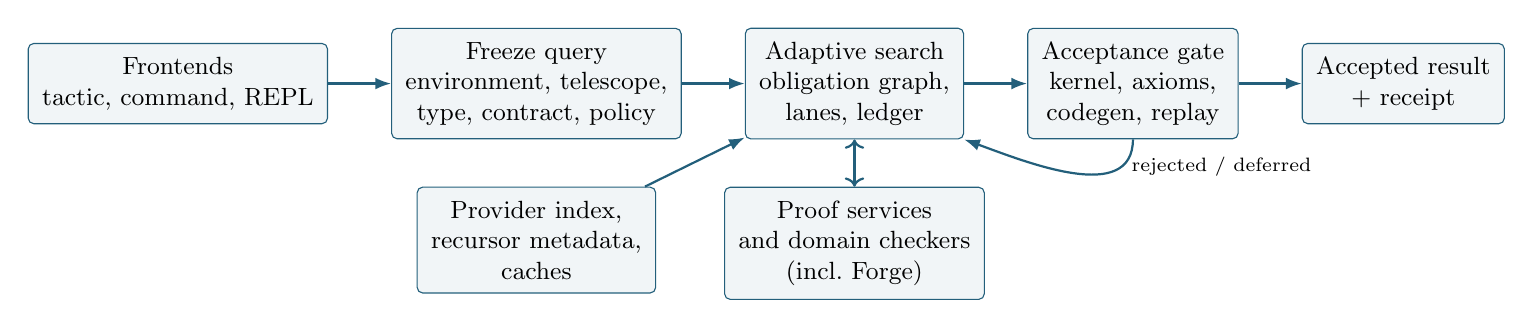
\begin{tikzpicture}[node distance=6mm and 8mm]
\node[box] (fe) {Frontends\\tactic, command, REPL};
\node[box, right=of fe] (fr) {Freeze query\\environment, telescope,\\type, contract, policy};
\node[box, right=of fr] (se) {Adaptive search\\obligation graph,\\lanes, ledger};
\node[box, below=of se] (pr) {Proof services\\and domain checkers\\(incl.\ Forge)};
\node[box, below=of fr] (ix) {Provider index,\\recursor metadata,\\caches};
\node[box, right=of se] (ga) {Acceptance gate\\kernel, axioms,\\codegen, replay};
\node[box, right=of ga] (out) {Accepted result\\+ receipt};
\draw[flow] (fe) -- (fr);
\draw[flow] (fr) -- (se);
\draw[flow] (se) -- (ga);
\draw[flow] (ga) -- (out);
\draw[flow] (ix) -- (se);
\draw[flow, <->] (se) -- (pr);
\draw[flow] (ga.south) to[out=-90,in=-20] node[pos=0.2,right,font=\scriptsize]{rejected / deferred} (se.south east);
\end{tikzpicture}}
\caption{The pipeline. Everything left of the gate is untrusted search; the gate adds nothing to what the kernel checks except refusal.}
\label{fig:pipeline}
\end{figure}

\section{The synthesis problem}\label{sec:problem}

\subsection{Queries and answers}

\begin{definition}[Frozen query]\label{def:query}
A frozen query is a tuple
\[
Q = (\E,\; U,\; \Gamma,\; T,\; \Phi,\; \Obs,\; \G,\; \Pol,\; \Bud)
\]
where $\E$ is the environment with its import identities and revision; $U$ is the universe-parameter context; $\Gamma$ is the ordered dependent local context, including \code{let} values and local instances; $T$ is the target with $\E;U;\Gamma \vdash T : \Sort\,u$; $\Phi$ is the optional contract with $\E;U;\Gamma, f{:}T \vdash \Phi(f) : \Prop$, taken as $\mathrm{True}$ when absent; $\Obs$ is a finite set of typed observations; $\G$ is the admitted construction grammar and provider inventory, stated in terms of constants and local terms rather than names; $\Pol$ is the trust and execution policy; and $\Bud$ is the resource policy\prov{all}.
\end{definition}

The query is elaborated once in the real project environment and frozen before search. Unknown identifiers are errors, not auto-bound implicits; universe parameters remain parameters and are never specialized; instance selection in the statement is part of the frozen question; and no metavariable owned by the caller may be assigned by search except through an explicit permission set returned as an atomic patch\prov{\Pn{5},\Pn{6},\Pn{8}}.

\begin{definition}[Answer]\label{def:answer}
A verified answer to $Q$ is a pair of judgments
\[
\E,\Delta;\,U;\,\Gamma \vdash t : T \qquad\text{and}\qquad \E,\Delta;\,U;\,\Gamma \vdash p : \Phi(t),
\]
where $\Delta$ is a finite list of generated auxiliary declarations accepted in dependency order under $\Pol$. The two judgments are kept separate rather than packed into a subtype, because $T$ may live in any sort and because a proof that specializes the candidate would describe a different program\prov{\Pn{2},\Pn{3},\Pn{5},\Pn{8}}.
\end{definition}

\begin{proposition}[Pointwise packaging]\label{prop:pointwise}
If $\Phi(f) \equiv \forall x{:}A,\, R(x, f\,x)$, then a term $g : \prod_{x:A}\{y : B(x) \,//\, R(x,y)\}$ yields $f := \lambda x.\,(g\,x).\mathrm{val}$ with $\forall x, R(x, f\,x)$, and conversely, constructively. The engine registers this as a checked transformation and uses the packed form to carry the contract into recursive branches (Section~\ref{sec:recursion}); it never pattern-matches on the syntax of $\Phi$ to decide correctness\prov{\Pn{1},\Pn{3},\Pn{9}}.
\end{proposition}

\subsection{Kinds of constraint}\label{sec:constraint-kinds}

Four kinds of behavioral input are supplied independently and are never silently converted into one another\prov{\Pn{1},\Pn{7}}:
\begin{itemize}
\item a \emph{hard contract} $\Phi$, which must be proved;
\item \emph{observations} $\Obs$: typed inputs with precondition evidence and expected outputs, or a proposition about particular inputs. They refute candidates and guide search; passing them establishes only themselves;
\item \emph{construction restrictions}: grammar predicates such as ``exclude \code{List.reverse}'', enforced on the transitive dependencies of the candidate, not on names;
\item \emph{preferences}: ranking signals such as ``prefer using every input'', which can never reject a correct program, since some correct programs must ignore inputs.
\end{itemize}

Leant's \code{:synth f : T where P} supplies a hard contract $P$ elaborated under the binder $f{:}T$; the baseline corpus contains no observations, restrictions, or preferences beyond this.

\subsection{The result algebra}\label{sec:results}

The nine proposals propose between five and nine result constructors. They are merged as follows; the internal representation carries orthogonal evidence fields, and the frontend may group constructors for display but the structured API preserves them\prov{\Pn{4},\Pn{6},\Pn{8},\Pn{9}}.

\begin{lstlisting}
inductive Outcome where
  | verified      (t : Accepted) (p : Accepted)  -- exact type and exact contract
  | typedOnly     (t : Accepted) (pending : Obligations)
  | testedOnly    (t : Accepted) (passed : Observations)   -- never satisfies a universal contract
  | refutedCandidate (t : Candidate) (q : Accepted)        -- proof of not (Phi t), or replayed counterexample
  | impossible    (q : Accepted)     -- proof of (t : T) -> Phi t -> False, or T -> False
  | fragmentUnderivable (fragment : Name) (cert : Checked) -- e.g. Kripke countermodel for IPC
  | grammarExhausted (grammar : Id) (ledger : Incompleteness)
  | budgetExhausted  (resumable : StateId) (ledger : Incompleteness)
  | unsupported   (feature : String)
  | infrastructure (error : String)
\end{lstlisting}

Each accepted object additionally records three independent flags, \code{kernelChecked}, \code{compiled}, and \code{evaluatedOnExamples}, together with the axiom inventory of the proof and the runtime-dependency inventory of the program (Decision~\ref{dec:three}). ``Best'' candidate means best among verified candidates under a declared cost model; ``minimal'' requires an exhausted cheaper prefix and is otherwise reported as ``lowest cost found under this schedule''\prov{\Pn{6},\Pn{8}}.

The baseline mapping is: Leant's displayed candidates correspond to \code{verified} (type-only queries have $\Phi = \mathrm{True}$, so the contract proof is trivial); ``provably uninhabited'' corresponds to \code{impossible} or \code{fragmentUnderivable}; ``no term found'' corresponds to \code{budgetExhausted} or \code{grammarExhausted}; ``none passed'' corresponds to \code{refutedCandidate} results with no \code{verified} result.

\subsection{Trust profiles}\label{sec:profiles}

Three policy profiles are recognized, each fixing an axiom allowlist for proofs and a separate runtime policy for programs\prov{\Pn{1},\Pn{3},\Pn{6},\Pn{9}}:
\begin{itemize}
\item \emph{strict constructive}: empty axiom inventory beyond explicitly accepted query assumptions; total, computable program; no \code{Classical.choice} on the computational path;
\item \emph{standard}: \code{propext}, \code{Quot.sound}, and \code{Classical.choice} permitted in proofs and erased transports, with actual use always reported; program still total and computable;
\item \emph{project-relative}: named project axioms permitted; results certified relative to them.
\end{itemize}
\code{sorryAx} is rejected in every profile. A result is never called ``axiom-free'' when it depends on \code{propext}; several prototypes' indexed \code{cases} did, and the receipts say so. The default profile for the baseline is \emph{standard}, which admits the classical candidates of \code{synth-manual}, labeled as such.

\section{Representations and search state}\label{sec:representations}

\subsection{Three representations, one type theory}

Every proposal converges on the same division of labor, in three tiers\prov{\Pn{3},\Pn{5},\Pn{8},\Pn{9}}.

\begin{enumerate}
\item \textbf{Semantic objects.} Native \code{Expr}, \code{Level}, names, binder information, local contexts, local instances, and the environment. These are authoritative and are never replaced by their pretty-printed form.
\item \textbf{The search plan.} A persistent, serializable record of search actions: introduce this binder; apply this exact provider occurrence with these universe instantiations and this spine prefix; split this scrutinee with this motive; instantiate this recursion schema; ask this proof service with this budget. Plan holes carry a stable identifier, a scope identifier, a native target closed over a dependency-closed telescope, and a role. The plan can be replayed against the frozen query to rebuild native state with fresh metavariable identifiers. It exists for resumption, caching, explanation, parallel transfer, and worker restart; it does not define a competing typing relation.
\item \textbf{Accelerators.} Discrimination-tree keys, type-head graphs, abstract domains such as list lengths and affine summaries, finite grammars, and solver encodings. Each is lossy and each declares its reconstruction boundary and its approximation polarity.
\end{enumerate}

\begin{invariant}[No naked open expressions cross a process boundary]\label{inv:serialize}
Raw \code{MVarId} and \code{FVarId} are never durable. A task shipped to another process or session is a closed plan over an ordered telescope with scope-stable binder positions, exact level and constant names, an environment fingerprint, and a protocol version. The receiver reopens it with fresh identifiers and rechecks; a mismatched fingerprint rejects the package rather than reinterpreting it\prov{\Pn{4},\Pn{8},\Pn{9}}.
\end{invariant}

Within one worker, native snapshots (\code{Meta.saveState}/\code{restore}) are the fast path. A production engine mixes two profiles: hot branches keep a materialized native checkpoint; cold branches are stored as a checkpoint plus the plan suffix needed to rematerialize them, bounding memory\prov{\Pn{5}}.

\subsection{Origin record and environment epochs}

The frozen query is stored as an immutable \emph{origin record}: toolchain identity, imported module identities, environment revision, the closed telescope, $T$, $\Phi$, the component policy, the axiom and execution policy, and the semantic options in force (transparency, active local instances, coercion configuration, grammar restrictions). Fingerprints locate cache entries; they never replace structural revalidation\prov{\Pn{9}}.

A worker owns an \emph{environment epoch}. Every handle, snapshot, cache entry, provider index, and proof-service reply is stamped with the epoch in which it was made. An undo, a \code{:reset}, an import change, or a worker restart bumps the epoch and invalidates everything stamped with the old one. Leant's session model, in which \code{:reset} and declaration replay change the environment mid-transcript, maps directly onto epochs\prov{\Pn{1},\Pn{6},\Pn{7}}.

\subsection{Branch state and the obligation graph}\label{sec:obligation-graph}

\begin{definition}[Branch state]\label{def:branch}
A branch is $S = (O, M, r, H, D, K, R, \Obs_S, \rho, c)$: the origin record; the native metavariable and elaboration state; the root program and root contract-proof expressions; the set of open obligations; the dependency graph over them; the delayed-constraint store; the set of recursive-call capabilities in scope; the branch-local observation bank version; the plan suffix that regenerates the branch; and the branch cost vector\prov{\Pn{2},\Pn{3},\Pn{7},\Pn{9}}.
\end{definition}

Each obligation $h \in H$ records its goal metavariable, its local context $\Gamma_h$, its target $T_h$, its residual contract $\Phi_h$ if any, and a \emph{role}: program value, type or universe argument, instance evidence, index equality, contract proof, termination proof, invariant, or reconstruction check. Roles guide scheduling; they never affect typing.

The dependency graph has an edge $h_1 \to h_2$ whenever assigning a metavariable reachable from $h_1$ can change the type, context, admissibility, or residual contract of $h_2$. Reachability is computed over local declaration types and values, delayed constraints, instance arguments, and the contract, not only over syntactic occurrence; read and write footprints are conservative over-approximations. Obligations that can assign metavariables reachable from one another form \emph{coupled clusters}, the strongly connected components of $D$, and are scheduled as units. A constructor application whose fields depend on one another is one hyperedge, not a sequence of independent children\prov{\Pn{3},\Pn{6},\Pn{7},\Pn{8}}.

\begin{invariant}[Branch ownership]\label{inv:ownership}
Every unassigned metavariable belongs either to the frozen ambient problem or to exactly one branch lineage. A branch may assign only its own search metavariables; it may not change the frozen statement, specialize the query's universe parameters, publish declarations, or reuse another branch's assignment without a checked context embedding. When Leant2 runs inside an unfinished proof, the permitted assignment set for ambient metavariables is computed at freeze time and any delta is returned as one atomic patch\prov{\Pn{6},\Pn{7},\Pn{8}}.
\end{invariant}

\begin{invariant}[Scope closure, type coherence, dependency coherence, evidence ownership]\label{inv:four}
Every obligation's target is closed under its own context; an unresolved proof obligation remains an obligation rather than being weakened; assigning a metavariable invalidates any observation, index entry, or summary whose recorded support depends on it; and a proof, counterexample, or summary is meaningful only for the exact expression, context, contract, and policy it was produced for\prov{\Pn{8}}.
\end{invariant}

\section{Transactional search}\label{sec:transactions}

\subsection{The atomic attempt}

The fundamental operation is the atomic attempt: snapshot all state the rule may write, run the rule, recurse on the rule's new obligations \emph{prepended to the remaining obligations of the branch}, and commit only if that whole continuation succeeds; otherwise restore, retaining only tagged diagnostics and the ledger charges\prov{all}. The prototype form, common to all nine packages up to naming, is:

\begin{lstlisting}
partial def solve (fuel : Nat) : List MVarId -> SearchM Bool
  | []      => pure true
  | g :: gs => do
    if fuel = 0 then return false
    if <- g.isAssigned then return <- solve fuel gs
    for rule in rulesFor g do
      let saved <- saveState
      try
        let children <- rule.apply g          -- may assign metavariables shared with gs
        if <- solve (fuel - 1) (children ++ gs) then return true
      catch e => if isInterrupt e then throw e  -- never swallow cancellation
      restore saved
    return false
\end{lstlisting}

The production engine replaces recursion by explicit \emph{cursor frames} (focused obligation, siblings, saved state, rule family, next alternative, cost allowance) so that a branch can be suspended, resumed, serialized, and scheduled fairly, but the semantics of the attempt are those above\prov{\Pn{6},\Pn{8}}.

\begin{invariant}[Commit criterion]\label{inv:commit}
A subgoal's solution may be memoized as an alternative, but its assignments become irrevocable only when every dependent obligation in the enclosing coupled cluster has been discharged or the generalization has been independently justified. An AND-node is a joint obligation with correlated substitutions, not a Cartesian product of independent first answers\prov{\Pn{2}}.
\end{invariant}

What a snapshot must cover depends on the rule. A pure \code{MetaM} rule needs the metavariable context and caches. A rule that elaborates syntax needs the elaborator state, postponed synthetic metavariables, local instances, and diagnostics. A rule that creates declarations needs an environment transaction, and such rules are staged: they run against a scratch environment and are committed only by the acceptance gate\prov{\Pn{2},\Pn{5},\Pn{9}}.

\subsection{Rule outcomes and blocked states}

A rule returns one of \code{progress} (new obligations, changed holes), \code{solved}, \code{blocked}, \code{rejected} (optionally with a certificate), \code{unsupported}, or \code{interrupted}. Three kinds of ``blocked'' are distinguished and none is a contradiction: blocked on assignments (a delayed equation or instance goal waiting for named metavariables), unsupported by this lane (with the continuation preserved for another lane), and yielded for budget (with the charged work and the continuation)\prov{\Pn{2},\Pn{6}}. Delayed constraints carry dependency stamps and are woken only when a relevant metavariable is assigned; a flex-rigid equation that becomes a pattern, an instance goal whose output parameters become ground, and a contract that reduces after an assignment are all wake-up events\prov{\Pn{4},\Pn{6},\Pn{9}}.

Unification is a service, not a completeness oracle. Its results are classified as deterministic progress, blocked, speculative, or mismatch; a rigid-head mismatch rejects an alternative cheaply; a budget failure or a stuck higher-order equation is unknown and never enters a negative cache\prov{\Pn{3},\Pn{7}}.

\subsection{Joint mode and frozen mode}\label{sec:joint-frozen}

Proof services are invoked in one of two modes, and the modes are distinct APIs\prov{\Pn{1},\Pn{2},\Pn{7}}.
\begin{itemize}
\item In \emph{joint mode} a proof attempt may assign program holes within the current transaction. Solving $?m = n + 1$ by unification determines the witness. Any such assignment is returned as part of the branch's construction choice, is subject to the commit criterion, and must respect the executable policy.
\item In \emph{frozen mode} the candidate is closed and the service may not replace or specialize it. A proof of $\neg\Phi(t)$ rejects exactly $t$ in exactly this context. A verifier that could mutate its candidate would produce receipts about a different program.
\end{itemize}
A reopened data choice creates a new candidate identity; evidence transfers between identities only through an explicit checked equality with contract transport\prov{\Pn{4}}.

\section{Adaptive scheduling}\label{sec:scheduling}

Decision~\ref{dec:single-engine} removes Leant's engine switches and settings. What replaces them is a single scheduler that runs a \emph{portfolio of lanes} over one obligation graph and adapts its allocation to the query and to progress. This section merges the scheduling designs of the nine proposals into that one engine.

\subsection{Lanes}

A lane is a policy over the same search actions; lane identity never changes what a candidate means. The initial lanes are\prov{\Pn{1},\Pn{2},\Pn{7},\Pn{9}}:
\begin{itemize}
\item \emph{exact reuse}: locals, projections of known locals, and direct heads that already have the target type;
\item \emph{focused construction}: introductions, constructors, and application spines over locals and the goal's own constructors;
\item \emph{library composition}: indexed retrieval and demand-directed composition of environment providers (Section~\ref{sec:library});
\item \emph{dependent elimination}: case splits and transports (Section~\ref{sec:elimination});
\item \emph{recursion}: schema instantiation, motive generalization, carriers (Section~\ref{sec:recursion});
\item \emph{constructive propositional}: a terminating focused calculus over a reified propositional fragment with a certificate for non-derivability (Section~\ref{sec:classical});
\item \emph{classical}: \code{Classical.em} and \code{Classical.byContradiction} as explicit providers, enabled by policy after the constructive lane has returned a certificate;
\item \emph{proof}: the portfolio of Section~\ref{sec:proof-services};
\item \emph{behavioral}: counterexample-guided refinement and domain checkers (Section~\ref{sec:cegis});
\item \emph{reference}: a conservatively enumerated fallback grammar with increasing cost bounds, which prunes only with a checked certificate.
\end{itemize}
Every lane exposes a bounded step, \code{step : Origin -> Task -> Quantum -> WorkerM StepResult}, returning a continuation, proposals, and a work delta. Every generator is a finite-step cursor, not a lazy stream\prov{\Pn{3},\Pn{9}}.

\subsection{Allocation}

Within a branch, the next obligation is chosen by \emph{pressure}\prov{\Pn{5},\Pn{6}}:
\[
\begin{aligned}
\mathrm{pressure}(h) = {}& a\cdot\mathrm{dependentUses}(h) + b\cdot\mathrm{knownIndexTests}(h) \\
& + c\cdot\mathrm{behaviorConstraints}(h) - d\cdot\mathrm{estimatedBranching}(h),
\end{aligned}
\]
with aging to prevent starvation. A cheap proof field that determines a data field is preferred over the data field (proof-first); when no such field exists, witness-first search with continuation backtracking is retained. Coupled clusters are scheduled as units.

Across branches the scheduler runs weighted round-robin over lane families with best-first order within a lane. The priority of a job $j$ is
\[
s(j) = g(j) + \lambda_h\,\hat h(j) + \lambda_p\,\hat p(j) + \lambda_d\,\mathrm{duplication}(j) - \lambda_r\,\mathrm{relevance}(j),
\]
where $g$ is charged cost, $\hat h$ an estimate of remaining construction, $\hat p$ an estimate of proof debt, and the last two terms penalize syntactic near-duplicates and reward obligations that mention rigid heads and concrete observations. This is a heuristic order, explicitly not an admissible A$^*$ heuristic\prov{\Pn{1},\Pn{5}}.

Fairness is guaranteed structurally, not by weights. The reference lane holds a reserved nonzero share of quanta (one in eight by default) and enumerates admitted plans by a \emph{diagonal schedule} over the tuple (lane, expression-cost bound, recursion-scheme bound, verification allowance), increasing the sum with deterministic ties. Within a tier the heuristic queue is complemented by a reserved FIFO stream so that the fairness claim is honest. Queue caps in fast lanes are permitted, and every dropped state is recorded as an incompleteness event in the ledger rather than treated as a refutation\prov{\Pn{2},\Pn{5},\Pn{7},\Pn{9}}.

Verification is scheduled alongside generation. A candidate whose contract proof returns unknown keeps a verification continuation with an increasing proof budget in an \emph{unresolved queue}; a bare rejection never shrinks the raw candidate window; a successful-result quota is not a raw-candidate quota\prov{\Pn{7},\Pn{8}}.

\subsection{How the adaptive engine replaces Leant's settings}\label{sec:adaptive}

Leant exposes \code{synth-steps}, \code{synth-window}, \code{synth-verify}, \code{synth-shown}, \code{synth-budget}, \code{synth-timeout}, \code{synth-classical}, \code{synth-library}, \code{synth-providers}, and \code{synth-engine}. Leant2 has none of them at first. The corresponding behaviors are internal:
\begin{itemize}
\item \emph{engine}: the lane portfolio is always active; lane weights adapt to the query shape (propositional goals raise the constructive lane; goals whose head is a library inductive raise library composition; contracts raise the behavioral lane) and to progress (a lane that has yielded nothing in its last $k$ quanta has its weight halved, subject to the reserved share);
\item \emph{steps and budget}: the work ledger has a global wall-clock deadline derived from the query's size and a logical work budget that grows by the diagonal schedule; there is no per-query knob;
\item \emph{window, verify, shown}: candidates are streamed to the frontend as they are accepted; the number displayed is a frontend concern; verification is scheduled per candidate as above and never capped by a count;
\item \emph{classical}: the classical lane is enabled by the \emph{standard} profile after the constructive lane has produced a certificate, so classical candidates appear later and labeled, which is the behavior Leant's default configuration approximates;
\item \emph{library and providers}: retrieval tiers widen automatically (Section~\ref{sec:library}); provider discovery is always on, and a result records which tiers were used.
\end{itemize}
Because allocation adapts, Leant2 may find candidates that Leant's fixed-window configurations missed (the three ``no term found'' controls and the two ``none passed'' verification-window controls of the baseline are examples), and it may rank candidates differently: the cost vector of Section~\ref{sec:ranking} replaces Leant's engine-specific ranking. Both are permitted by Definition~\ref{def:baseline}.

\subsection{Ranking and multiple answers}\label{sec:ranking}

The cost of a candidate is a structured vector, not a scalar\prov{\Pn{2},\Pn{3},\Pn{6},\Pn{8}}:
\[
\begin{aligned}
(&\text{policy violations},\ \text{term size},\ \text{eliminations},\ \text{recursion shape},\\
 &\text{transports},\ \text{nonlocal providers},\ \text{proof size},\ \text{runtime estimate}).
\end{aligned}
\]
The first component is an admission constraint. Candidates are ranked lexicographically by a declared profile (small source by default), and a small Pareto frontier of behaviorally distinct candidates is exposed rather than the first result only. Diversity is counted over native terms modulo checked equivalence, not over printed strings; two candidates that agree on all observations are presented as distinct unless a checked equality merges them. ``Use every input'' is a preference, not a filter.

\subsection{Resource limits and determinism}

Three independent controls apply: logical work budgets (rule applications, unification steps, normalization steps, proof tasks, solver calls, candidate evaluations), wall-clock deadlines, and process-level limits (memory, output size, external process lifetime). Counters are monotone and charged even after rollback (Decision~\ref{dec:ledger}). Per-rule limits yield suspended branches; raising a proof budget never regenerates earlier terms. A deterministic mode fixes ordering and seeds so that a transcript replays exactly; a performance mode returns the first result from parallel workers and records which lane produced it\prov{\Pn{3},\Pn{4},\Pn{9}}.

Parallelism is restricted to closed request slices: whole lanes, candidate verifications, and connected components of the dependency graph with an independence certificate (disjoint owned metavariables, disjoint synthetic obligations, unchanged shared rigid context). Workers exchange closed plans and certificates, never live metavariable contexts\prov{\Pn{1},\Pn{9}}.

\section{Native construction}\label{sec:construction}

The construction calculus is bidirectional. Checking $\Gamma \vdash e \Leftarrow T$ drives introductions from the expected type; inference $\Gamma \vdash n \Rightarrow T$ extends heads (locals, constants, projections) by spines and drives eliminations. Rules are labeled as \emph{checked transformation}, \emph{grammar-preserving normalization}, or \emph{heuristic proposal}, and a fairness lane retains the alternatives that aggressive focusing drops\prov{\Ref{3},\Ref{6},\Ref{9}}.

\subsection{Introductions}

For a target that weak-head-normalizes to $\prod_{x:A} B(x)$, introduce a fresh local preserving binder information (explicit, implicit, strict-implicit, instance-implicit). Introduction is existence-preserving for every binder kind, including type parameters, indices, and instance arguments, so it is the default focusing policy for function targets. It does not yield the smallest term: an existing function of the target type must also be considered, so a cheap \emph{exact-term lane} runs before eta-expansion, but a cheap inhabitant never suppresses contract-sensitive alternatives\prov{\Ref{3},\Ref{4},\Ref{5}}.

For an inductive target, enumerate all constructors rather than committing to the first; freshen the constructor's universe levels, instantiate parameters, and unify the result with the target in one transaction. An index equation that is inconsistent rejects the constructor; one that is merely blocked keeps it and records a delayed constraint. In dependent pairs and subtypes, the data field remains a choice point until every dependent field and the contract are satisfied; proof irrelevance may deduplicate proofs of a fixed proposition, never data\prov{\Ref{1},\Ref{6}}.

\subsection{Application spines}\label{sec:spines}

\begin{definition}[Spine expansion]
For a head $c : \prod_{a_1:A_1}\cdots\prod_{a_k:A_k(\vec a_{<k})}\,R(\vec a)$: freshen the universe parameters of this occurrence; for each admissible prefix length $j \le k$, in a fresh transaction, create owned holes $?a_1,\dots,?a_j$ in telescope order with exact binder information, and unify the residual type $\prod_{a_{j+1}}\cdots R$ with the target; keep the full argument vector so that later arguments can constrain earlier ones; classify each hole by role; discharge determined instance and proof arguments cheaply; suspend blocked constraints with dependency stamps; and yield the application together with its whole coupled continuation\prov{\Ref{2},\Ref{3},\Ref{6},\Ref{8},\Ref{9}}.
\end{definition}

Partial applications are admitted because a useful application length changes after reduction or when a type variable is instantiated by a function type. Repeated use of one head is allowed. The prototypes build this on \code{MVarId.apply} with \code{newGoals := .all} (original argument order, which forces witness-first backtracking to be tested) and \code{approx := false}; the design treats \code{apply} as a first adapter and differential-tests any optimized spine planner against it\prov{\Ref{2},\Ref{3},\Ref{6}}.

Local providers keep their exact free-variable identities and universes; only global constants are freshened per occurrence. Named universe parameters of the query are rigid; fresh level metavariables of library constants are flexible; there is no implicit universe lifting and no lowering of a polymorphic query to \code{Type 0}\prov{\Ref{1},\Ref{2},\Ref{4}}.

\subsection{Known-major projections}

Applying \code{Sigma.snd} to an unknown pair leaves an unknown family and an unknown major premise. Instead, projections are first-class search actions over \emph{known} locals: enumerate \code{Expr.proj} over local structure values using structure metadata, infer the exact dependent type, and match. This fixed a real regression ($p : \Sigma_n \mathrm{Fin}(n+1) \vdash \mathrm{Fin}(p.1 + 1)$) generically, and projection-first ordering also fixed a heartbeat exhaustion caused by constructor growth before projections in another prototype\prov{\Ref{1},\Ref{5}}.

\subsection{Polymorphic and higher-rank instantiation}\label{sec:polymorphism}

Higher-rank arguments are Pi-typed argument holes and are constructed by introduction; there is no rank-N approximation. Type-valued holes are filled by a staged \emph{type-invention ladder}\prov{\Ref{1},\Ref{2},\Ref{6},\Ref{9}}:
\begin{enumerate}
\item types forced by unification with the rigid target;
\item expected-type-directed construction of polymorphic arguments (introduce the binder rather than enumerate monotypes);
\item a bounded, cost-ordered \emph{type frontier}: types in the telescope, output, and contract; types of locals and of provider domains; small products, sums, sigma and function types over those; registered carrier templates;
\item quantified types and accumulator carriers, with a separate size cost.
\end{enumerate}
Pool exhaustion is a missed instantiation, not impossibility. Stuck higher-order equations are postponed, then bounded-instantiated with small lambda, projection, and application templates, each rechecked by Lean; there is no general higher-order unification. The Church and rank-N fixtures of the baseline are the primary regression set for this ladder.

\subsection{Instances and dictionary identity}\label{sec:instances}

Two modes must not interfere. In \emph{canonical instance mode}, instance obligations are Lean's own resolution, delayed until their input parameters are known and woken on assignment. In \emph{explicit dictionary mode}, a dictionary is data: local instances are named providers, the actual dictionary expression is stored at each method occurrence, and search may backtrack over dictionary choices. Two dictionaries of the same class type are never interchangeable without a proved equivalence; only \code{Prop}-valued classes enjoy proof irrelevance. Cache keys and candidate identity include dictionary payloads. The fixture in which the second of two \code{Inhabited Nat} values must be selected because the contract says so is a permanent regression\prov{\Ref{1},\Ref{3},\Ref{5},\Ref{6},\Ref{8}}. Leant2 never manufactures global instances.

\subsection{Normalization and equality}

Normalization is controlled work: memoized weak-head normalization, a small transparency ladder with per-operation budgets, escalation on failure, and charges that survive rollback. Definitional equality is an operation, not a canonicalizer: there are no pretty-printed normal-form cache keys. The order for an index mismatch such as $\mathrm{Vec}\,A\,(n+m)$ against $\mathrm{Vec}\,A\,(m+n)$ is cheap definitional equality, then registered proof-producing normalizers, then a bounded equality proof $q : n+m = m+n$ followed by an explicit transport along the equality recursor with a Lean-checked motive; never a raw cast, and never index erasure\prov{\Ref{3},\Ref{4},\Ref{6},\Ref{8}}.

\subsection{The constructive propositional lane and classical candidates}\label{sec:classical}

Leant's baseline includes propositional goals proved constructively (\code{synth-basic}, \code{synth-manual}, \code{synth-prove}) and, with \code{synth-classical on}, classically. It reports \code{forall p : Prop, p or not p} as ``provably uninhabited'' because Djinn's LJT search found no derivation. Leant2 reproduces this capability with two lanes and one rule.

The \emph{constructive propositional lane} reifies the propositional fragment of a goal (connectives $\to,\wedge,\vee,\neg,\leftrightarrow,\bot,\top$ over atoms that are opaque Lean propositions or types), runs a terminating focused calculus over it, and returns either a Lean proof term or a checkable certificate that no derivation exists in that fragment. The certificate is a finite Kripke countermodel, checked by recomputing forcing, as in Forge's extension round \cite{forge}. The result is \code{fragmentUnderivable}, with the fragment named, and it is never promoted to \code{impossible}\prov{\Ref{1},\Ref{4},\Ref{6},\Ref{8}}.

The \emph{classical lane} adds \code{Classical.em}, \code{Classical.byContradiction}, and \code{Decidable.em} as explicit providers. It is enabled by the \emph{standard} profile and scheduled after the constructive lane has returned a certificate, so that constructive candidates are found first and classical ones are labeled by their axiom inventory. For the baseline this yields the classical candidates of \code{synth-manual} and, for \code{forall p : Prop, p or not p}, both a fragment certificate and a labeled classical candidate.

\section{Dependent elimination}\label{sec:elimination}

Case analysis is a motive-construction problem, delegated to Lean's own machinery behind a wrapper that returns the branch goals, the old-to-new local mapping, and any transport obligations\prov{\Ref{3},\Ref{4},\Ref{6},\Ref{8},\Ref{9}}.

\begin{enumerate}
\item Compute the dependency closure of the scrutinee $x : I\,\vec p\,\vec i$: every later local whose type or value mentions $x$, its indices, or a selected dependent.
\item Generalize the closure into the motive, preserving order; inspect the real eliminator and its result-sort restriction; build the motive over the indices and the scrutinee.
\item Instantiate each constructor branch with its fields and index equations; reintroduce the dependent context with transformed types; record the branch-to-parent substitution.
\item Discharge impossible constructor and index combinations only by checked evidence: unification contradiction, no-confusion, or a proved local contradiction. Record for each removed branch whether it was removed by kernel-checked contradiction, by a trusted exact-fragment theorem, or by heuristic omission; only the first two support coverage claims.
\item Reconstruct the eliminator application.
\end{enumerate}

Scrutinee selection prefers locals that occur in target indices, that a discriminating contract or observation demands, or that block reduction. Split history is tracked by discriminant identity, so repeated splitting of a recursive input is recognized as bounded unrolling and not as recursion. Elimination restrictions are enforced natively: \code{False} eliminates anywhere; \code{Nonempty A} is not an executable \code{A}; \code{Exists} is not a computational pair; quotients require a respect proof through their registered lift. Decidable conditionals require an admitted \code{Decidable} instance and a checked link between the condition and the branch facts\prov{\Ref{2},\Ref{4},\Ref{7}}.

Every prototype that eliminated an indexed family with \code{cases} picked up \code{propext}; the receipts report it, and the strict profile treats it as a policy decision rather than hiding it.

\section{Library composition and carrier invention}\label{sec:library}

\subsection{The provider index}

A persistent index is built at import over declaration types: identity, universe parameters, telescope, weak-head result shape, argument heads, constructor or projection role, computational-versus-proof classification, and registered specification lemmas. The index is a discrimination tree over normalized result heads with mandatory wildcard and reducible-head buckets; it may over-return but never silently under-returns, and an intentionally narrowed query is never negative evidence\prov{\Ref{4},\Ref{5},\Ref{8},\Ref{9}}.

Retrieval widens in tiers, each recorded in the result: locals and local dictionaries; the goal's own constructors and projections; explicitly requested providers; registered project components and tagged \emph{synthesis lemmas}; nearby namespaces and imports; a budgeted broad scan. A fixed cap such as fifty providers is a heuristic, never ``exhaustive''\prov{\Ref{1},\Ref{9}}.

\subsection{Component recipes and the join}

A component is a recipe $(\Delta \vdash e : \sigma,\ \text{contract lemmas},\ \text{cost},\ \text{provenance})$ with $\Delta$ the dependency-closed telescope. Reuse under $\Gamma$ requires a telescope substitution $\rho : \Delta \to \Gamma$ applied uniformly to $e$, $\sigma$, and the contracts, followed by a native recheck. Forward synthesis stores cheap components in a typed shared DAG; backward synthesis demands result types; a \emph{join} matches demanded premises against stored components and propagates assignments across the whole application\prov{\Ref{6},\Ref{7}}.

A \emph{demand graph} from target holes and observations yields, per demand, a \emph{candidate context slice}: the locals mentioned in the type, contract, and constraints plus a bounded predecessor closure. The slice is searched first and the full context second; slice solutions are transported by explicit weakening and rechecked. This is the direct response to Leant's indexing diagnostic, in which a handler found standalone is missed in the full context\prov{\Ref{7},\Ref{8}}.

\subsection{Providers with contracts}

A provider is an exact term plus useful theorems: the declaration, its universe telescope and binder structure, result-head keys, instance dependencies, a use policy, and \emph{specification entries} naming theorems $\forall x,\ P(x) \to Q(x, g(x))$ that relate the operation to its inputs and outputs. Entries are checked at registration and never trusted as annotations; a summary must name its justifying theorem and instantiate it at the same occurrence. Multiple specifications per provider are selected by the demanded observation (length, order, multiset). Provider exclusion follows declaration dependencies, not namespace blacklists, so a withheld reference implementation cannot be retrieved through an alias\prov{\Ref{3},\Ref{5},\Ref{8},\Ref{9}}.

Parametricity is a ranking heuristic and a template source, never a pruning axiom: Lean's axioms admit nonparametric functions\prov{\Ref{2},\Ref{5}}.

\subsection{Carrier invention}\label{sec:carriers}

When an eliminator or fold is applied and the continuation still consumes an argument after the traversal, the carrier is not the result type. The engine tries, in increasing structural cost, the carrier grammar
\[
C ::= R \;\mid\; I \to C \;\mid\; C_1 \times C_2 \;\mid\; \mathrm{Option}\,C \;\mid\; \Sigma d{:}D,\, C(d),
\]
seeded by demanded types, with three demand rules: \emph{parameter postponement} (a parameter consumed after the traversal becomes the domain of a function-valued carrier), \emph{result pairing} (two demanded summaries become a product), and \emph{accumulator generalization} (a changing argument becomes an accumulator). Generalization is \emph{behavioral}: it includes arguments whose values change across calls, not only those the type depends on. The worked trace shared by four proposals is defaulted indexing, \code{List A -> Nat -> Option A}, as \code{foldr} with carrier $\Nat \to \mathrm{Option}\,A$, $z(i) = \mathrm{none}$, $s(x,r)(0) = \mathrm{some}\,x$, $s(x,r)(k+1) = r(k)$; one proposal checked a hand-supplied instance of it, none discovered it automatically\prov{\Ref{1},\Ref{4},\Ref{5},\Ref{7},\Ref{8},\Ref{9}}.

Base and step are attempted jointly with the outer continuation; failures are memoized only under the full context, motive, and bound. Typed anti-unification of repeated residual obligations proposes shared helper types and let-bound helper holes solved under the intersection of scopes\prov{\Ref{1},\Ref{2},\Ref{8}}.

\section{Recursion}\label{sec:recursion}

Recursion is the area where the nine proposals agree most closely on design and have demonstrated the least. Every recursive definition in every prototype was hand-supplied; the tactics filled branch bodies. This section states the consensus design and marks its unimplemented parts.

\subsection{Routes, in order}

Given a target whose telescope contains an inductive argument, the recursion lane tries, in order\prov{\Ref{2},\Ref{3},\Ref{4},\Ref{5},\Ref{8},\Ref{9}}:
\begin{enumerate}
\item a permitted library combinator with a matching specification entry (\code{map}, \code{foldr}, \code{foldl}, option combinators, registered recursors);
\item a nonrecursive eliminator or fold already in the local context, including Church-encoded values with function-valued carriers (Section~\ref{sec:carriers});
\item a \emph{structural schema} generated from the recursor metadata of the input type;
\item a strengthened or accumulator-generalized structural schema;
\item a well-founded schema over an explicit measure.
\end{enumerate}
Mutual recursion is a jointly synthesized strongly connected component over a tagged sum with a shared termination argument; nested inductives use their actual recursors; both are later extensions\prov{\Ref{3},\Ref{8}}.

\subsection{Schemas and capabilities}

\begin{definition}[Recursion schema]
A schema records the function telescope, the decreasing argument, the result family (motive) $M(\vec i, x)$, one branch per constructor with its fields and index equations, the set of \emph{recursive-call capabilities} available in each branch, the termination obligations, and the lowering plan\prov{\Ref{4},\Ref{7},\Ref{9}}.
\end{definition}

\begin{invariant}[Recursive calls are capabilities]\label{inv:capabilities}
A branch never contains an unrestricted local $f : \forall x, T(x)$. A recursive call is available only as $\mathrm{rec} : \prod_{y:D}\,\prec(y,x) \to M(y)$, where the decrease evidence is a constructor field for structural recursion or an obligation $\mu(y) < \mu(x)$ for well-founded recursion. The obligation is synthesized or the call is rejected; the program is never rejected because a measure failed\prov{all}.
\end{invariant}

The failed first run of one prototype, in which unfiltered implementation-detail locals exposed the provisional definition and Lean rejected the resulting cycles, is the empirical reason for this invariant. The acceptance gate additionally audits the dependency graph of the declaration bundle for provisional self-reference\prov{\Ref{2}}.

\subsection{Motive construction}

\begin{definition}[Motive by dependency-closed generalization]
Choose the discriminant $z : D(\vec p, \vec i)$. Partition the surrounding variables into fixed parameters and generalized arguments, closed under dependence and under behavioral change (arguments whose values differ between the call and the recursive call). The candidate motive is
\[
M(\vec i, z) = \prod \Delta(\vec i, z).\; R'(\vec i, z, \Delta),
\]
checked by Lean at the recursor's sort. The schema instantiates the recursor, exposes the method holes and induction hypotheses, translates the residual contract per branch, and requires a checked \emph{final specialization} back to the original target\prov{\Ref{2},\Ref{5},\Ref{6},\Ref{9}}.
\end{definition}

Motives are tried on a complexity ladder: the direct result family; generalize the dependent arguments; small subsets of the changing arguments; accumulator and invariant templates. The worked examples common to the proposals are \code{Vec.map} with $M(n, xs) = \mathrm{Vec}\,\beta\,n$, \code{Vec.zip} with $M(n, xs) = \mathrm{Vec}\,\beta\,n \to \mathrm{Vec}\,(\alpha\times\beta)\,n$, vector lookup with $M(n, xs) = \mathrm{Fin}\,n \to \alpha$, and accumulator reversal with the motive quantified over the accumulator. Motive-subset search is exponential in the number of changing arguments; the mitigation is the ladder plus \emph{failure-directed generalization}: classify why an induction hypothesis cannot be applied and compute the smallest dependency-closed telescope extension that repairs it\prov{\Ref{2},\Ref{6}}.

\subsection{Proof-carrying motives}\label{sec:certified-motive}

The central idea for program-and-proof co-synthesis appears in all nine proposals under different names (certificate algebras, refinement motives, certified recursion, packed motives): strengthen the motive so that the induction hypothesis carries correctness\prov{all}.

\begin{proposition}[Certificate-algebra composition]\label{prop:algebra}
Let $C(x) = \{y : B(x) \,//\, R(x, y)\}$. A native recursor application with motive $C$ and checked method terms yields $\prod_{x:D} C(x)$, hence an output satisfying $R$ for every input. For function-valued outputs the motive is $C(x) = \prod_{a:S}\{y : B(x,a) \,//\, R(x,a,y)\}$. The list instance is the checked theorem
\[
R([], z) \;\wedge\; \big(\forall x\,xs\,v,\ R(xs, v) \to R(x{::}xs, s(x,v))\big) \;\Rightarrow\; \forall xs,\ R(xs, \mathrm{foldr}\ s\ z\ xs).
\]
\end{proposition}

Each recursive branch receives the smaller output \emph{and} its local specification, so a contract failure backtracks into the branch choice rather than rejecting a finished term. The alternative route, synthesize then prove by induction on the checked equations, is kept as a portfolio alternative and is preferred when the contract is not pointwise. Two proposals checked hand-written instances (\code{certifiedMap} with a functional \code{MapRel}; \code{certifiedAppend}; \code{indexFold} with its universal correctness)\prov{\Ref{1},\Ref{5},\Ref{8}}.

\subsection{Accumulator invariants}

When a helper with an accumulator is needed, the invariant is a bounded synthesis subproblem, never an assumption. The grammar is built from the public relation, the accumulator variable, the available operations and their registered algebraic summaries, and known unit elements; each candidate yields initiation, preservation, and finalization obligations proved by the proof portfolio. The example shared by six proposals is $\mathrm{go}(xs, acc) = \mathrm{reverse}(xs) \mathbin{+\!\!+} acc$ for accumulator reversal; two of them proved the invariant by hand for the fold selected by a finite experiment, and none synthesized it\prov{\Ref{2},\Ref{3},\Ref{4},\Ref{6},\Ref{8},\Ref{9}}.

\subsection{Termination}

The well-founded schema is $F(x) = \mathrm{step}(x, \lambda y\,(h : y \prec x).\,F(y))$. Measures come from a finite grammar: natural-number arguments, registered size functions, structural sizes, bounded differences such as $n - i$ with truncated-subtraction semantics handled honestly, lexicographic tuples, and user-supplied relations. Each proposed call yields $\mu(y) < \mu(x)$ as an ordinary obligation; a schema is registered only after Lean's termination elaboration accepts it. Fuel is legal only when it is part of the interface or proved sufficient\prov{\Ref{1},\Ref{3},\Ref{5},\Ref{8}}.

\subsection{The kernel/compiler boundary}\label{sec:lowering}

Four prototypes independently produced an axiom-free recursor term that the code generator rejected (``code generator does not support recursor \code{T.rec} yet''). The consequence is a design rule\prov{\Ref{4},\Ref{6},\Ref{8},\Ref{9}}:

\begin{invariant}[Two products per recursion plan]\label{inv:lowering}
A recursion schema produces a logical reconstruction, used for proof, and an executable definition, lowered from the plan through the equation compiler with pattern equations and, when needed, \code{termination_by} and decrease proofs. If the two differ, the engine proves a correspondence theorem $\forall t,\ f_{\mathrm{eq}}(t) = f_{\mathrm{rec}}(t)$ and checks both, or proves the contract directly for the executable definition. The receipt records \code{kernelChecked} and \code{compiled} separately.
\end{invariant}

Lowering recovers the major argument, patterns, branch locals, capabilities, and generalized arguments from the plan, not from printed recursor text, and elaborates the result in a staging environment that contains only approved dependencies\prov{\Ref{6}}. The recursion-schema grammar tags each construction as genuine recursor, bounded unrolling, or nonrecursive, so that repeated case splits are not mistaken for recursion\prov{\Ref{5}}.

\subsection{Status}

Demonstrated: filling branch bodies inside hand-supplied structural skeletons on indexed vectors and lists; hand-written proof-carrying motives and their universal correctness theorems; the code-generator boundary. Not demonstrated: automatic schema generation, motive generalization, carrier discovery, invariant synthesis, measure synthesis, lowering. This is the gate that the roadmap of Section~\ref{sec:roadmap} treats as the decisive capability milestone\prov{\Ref{8}}.

\section{Behavioral constraints}\label{sec:behavior}

Behavioral information enters search from three directions: the type constrains shape, the contract propagates backward into holes, and observations and counterexamples constrain choices. None replaces the final proof\prov{\Pn{3},\Pn{9}}. The propagation rules, the refinement loop, and the pruning procedures are given as algorithms in Section~\ref{alg:behavior}; scheduling and caching in Section~\ref{alg:scheduling}; proof services and the gate in Section~\ref{alg:acceptance}.

\subsection{Contract decomposition}

A \emph{contract decomposer} takes the elaborated contract $\Phi$ and a construction step and returns local obligations together with a \emph{reconstruction term} proving that they imply the original. Each extracted view is tagged \emph{necessary}, \emph{sufficient}, or \emph{equivalent}, and the original $\Phi$ stays authoritative\prov{\Pn{2},\Pn{6},\Pn{8},\Pn{9}}. The initial library of decomposition rules is:
\begin{itemize}
\item lambda introduction: a pointwise $\forall x, \mathrm{Post}(x, f\,x)$ becomes $\mathrm{Post}(x, ?r)$ for the body hole (Proposition~\ref{prop:pointwise});
\item constructor application: a record invariant becomes projection equations on the fields;
\item decidable conditional: the postcondition splits under the guard and its negation;
\item provider application: a registered theorem $\forall a,\ P(a) \to Q(g(a))$ turns the demanded $Q$ into the \emph{sufficient} obligation $P(a)$ on the argument. Sufficiency does not license deleting arguments that fail $P$; they remain in another lane unless a necessity theorem exists;
\item conjunctions, constructor-aligned relations, and registered pre/postconditions.
\end{itemize}
Multi-call laws stay as higher-order obligations; an opaque higher-order provider stops propagation with a symbolic residual.

\subsection{Typed observations and residual evaluation}

An observation is a typed substitution into the input telescope, precondition proofs, an exact output observation, and an evidence policy. Dependent outputs are checked at their induced type; \code{Fin n} values carry their bound; dependent pairs generate the first field before instantiating the second's type; polymorphic functions are tested at several concrete types with distinct dictionary payloads. The default evaluator never runs effects; \code{IO} is never executed as a test; a timeout is unknown, never false\prov{\Pn{3},\Pn{6},\Pn{7}}.

Partial programs are evaluated \emph{residually}: evaluation proceeds until a hole and yields a typed residual (known constructors, closures, suspended applications, conditionals, named holes with observed arguments). A residual is a constraint on a particular use of the hole; multiple observed calls of one hole constrain one shared function, recorded in a hole-observation table keyed by hole and argument tuple so that $h(0) = 0$ and $h(0) = 1$ are recognized as inconsistent. Recursive-call outputs under a sketch are symbolic: a satisfying symbolic model alone is not a realizable program, and hard pruning requires a certified conservative completion abstraction, with contract-derived call assumptions scoped to contract-satisfying completions\prov{\Pn{2},\Pn{6},\Pn{7}}.

\subsection{Proof services}\label{sec:proof-services}

Proof obligations are discharged by a portfolio behind one adapter, in cost order: conversion and \code{rfl}; local assumptions; constructor proofs; \code{decide} by ordinary kernel reduction; curated \code{simp} with an explicit lemma set; \code{omega}; Forge's certificate checkers for cone, Farkas, affine-witness, recurrence, and conserved-invariant obligations \cite{forge}; \code{grind}; Aesop with query-specific rules; optional pinned Mathlib procedures. Induction is a deliberate schema choice coordinated with the recursion plan, not a generic proof step\prov{\Pn{1},\Pn{3},\Pn{5},\Pn{6},\Pn{9}}.

The adapter's contract is Forge's: save the full state before the worker, restore on any failure including resource limits, and on success instantiate the proof term and reject it if it contains \code{sorry}, mentions a free variable outside the goal's context, does not type-check against the original goal, or depends on an axiom outside the policy. A reply is one of \code{Proof} (with any permitted assignment patch, in joint mode), \code{Refutation}, \code{ReducedGoal} with a reconstruction proof, \code{Unsupported}, or \code{Unknown} with the budget consumed. A bare Boolean is not an adequate interface; a failed proof never falsifies a candidate; a result obtained under a branch guard discharges only guarded obligations\prov{\Pn{2},\Pn{3},\Pn{7}}. \code{native_decide} is not used for proofs; native evaluation may rank or propose but never certifies\prov{\Pn{8},\Pn{9}}.

Proof debt is scheduled: obligations carry cost and readiness, index and arithmetic obligations wake on relevant assignments, and heavy tactics are delayed until the computational holes they mention are assigned or exposed as witness choices\prov{\Pn{1},\Pn{5}}.

\subsection{Certified counterexample-guided refinement}\label{sec:cegis}

\begin{definition}[Verifier]
\[
\mathrm{verify}(t, \Phi) \in \{\mathrm{Proof}(p),\ \mathrm{Counterexample}(c),\ \mathrm{Unknown}(r),\ \mathrm{Failure}(e)\},
\]
where $c$ is a value of the actual input type with proofs of its preconditions and a checked violation. A counterexample enters the bank only after replay in Lean's exact interpretation; a solver model is a proposal until decoded and replayed; an evaluator timeout adds nothing\prov{\Pn{1},\Pn{4},\Pn{5},\Pn{8}}.
\end{definition}

The loop: choose the next candidate consistent with the bank; try to prove $\Phi(t)$; on unknown, schedule a counterexample search and keep the candidate in the unresolved queue at a larger proof tier; on a certified counterexample, add it to the bank, repartition the observation buckets, and wake suspended work; publish only through the acceptance gate. ``Failure of one is not success of the other'': a proof attempt and a counterexample search for the same candidate run as separate resumable tasks\prov{\Pn{6},\Pn{7},\Pn{9}}.

\begin{proposition}[Progress of finite counterexample search]
With $N$ candidates in a finite grammar, permanently retained valid counterexamples, and bank-consistent selection, at most $N$ rejections occur; unknown verdicts do not count as rejections\prov{\Pn{3},\Pn{8}}.
\end{proposition}

Finite domains are promoted to universal statements by an untrusted enumerator that proposes a literal and a kernel \code{decide} that proves the universal statement, decoupling synthesis time from proof size; the finite promotion theorem $(\forall x, x \in L) \wedge (\forall x \in L, R(x)) \Rightarrow \forall x, R(x)$ is checked once\prov{\Pn{6},\Pn{9}}. Two prototypes implemented finite Boolean CEGIS in Lean with the universal correctness proved by ordinary \code{decide}; one implemented a proof-carrying certifier \code{certify : Affine -> Option {c // Spec c.eval}} whose acceptance object is a Lean proof rather than a Boolean\prov{\Pn{7},\Pn{8},\Pn{9}}.

\subsection{Reversible observational buckets}

Candidates are grouped by their observation vector $\mathrm{obs}_\Obs(t) = (t(x_1), \dots, t(x_m))$. A bucket holds an active representative \emph{and} its members or their regeneration recipes; a new observation splits buckets and reactivates members; a second liveness rule rotates parked members even without new observations, since a parked candidate may have a shorter proof. Permanent merging is unsound: the Boolean pair (constant true, identity) agrees on \code{true} and differs on \code{false}, and three separate finite experiments showed that permanent deduplication on the initial bank loses the correct program (identity versus reverse; $x$ versus $y$ on $(0,0)$). Observational agreement is provisional and never an unrestricted cache equivalence; a restricted grammar may use a separately proved congruence with complete typed observations and cost-preserving representative replacement\prov{\Pn{1},\Pn{2},\Pn{3},\Pn{5},\Pn{9}}.

\subsection{Certified pruning}\label{sec:pruning}

\begin{proposition}[Sound sketch pruning]\label{prop:prune}
Let $P$ be a partial program with completions $\Comp(P)$ and let $A(P)$ be an abstract summary with $\{\Beh(t) : t \in \Comp(P)\} \subseteq \gamma(A(P))$. If some valid input $\rho_0$ has a defined observation for every completion, and a checked necessary condition $K$ on that observation satisfies $\gamma(A(P)) \cap K = \varnothing$, then no completion of $P$ satisfies $\Phi$\prov{\Pn{3},\Pn{5},\Pn{6},\Pn{8},\Pn{9}}.
\end{proposition}

A domain plugin implements Forge's \code{CertificateSpec} shape: a typed reification, an interpretation into Lean, a soundness theorem for its transfer rules, and refusal cases. Its replies are \code{Unsupported}, \code{RankingHint} (no logical authority), \code{NecessaryConstraint} with proof, \code{Counterexample} with validity evidence, or \code{NoCompletion} with a certificate and its exact grammar scope. Missing transfer rules yield top, never bottom; an under-approximation may produce witnesses but may never justify pruning; grammar identity is part of every certificate's applicability. Initial domains are list lengths and sizes, affine and linear arithmetic (Forge's checkers), constructor tags, bounded machine integers, and small multisets. One proposal proved the length-abstraction necessity and sufficiency for its fold grammar; another proved an exact five-list separator family for affine folds and generated twenty-seven universal contracts from it\prov{\Pn{3},\Pn{4},\Pn{5},\Pn{7}}.

External solvers have three distinct uses, each with its own validation: proposing sketch choices, proposing counterexample inputs, and proving theory obligations by a reconstructed certificate. \code{unsat} on an under-approximate encoding excludes only that encoding. Typed SMT sketches encode dependent holes either \emph{branch-expanded} (each witness alternative owns a specialized child grammar) or \emph{native-first} (the solver picks the witness and Lean generates the residual); untyped multiplexers are not used\prov{\Pn{2},\Pn{5},\Pn{6}}.

\section{Caching and equivalence}\label{sec:caching}

Three equivalences are kept apart: structural identity, checked semantic equality, and finite observational agreement\prov{\Pn{8}}.

Cache keys include the environment epoch and provider policy, the canonical dependent context preserving \code{let} values and instance identities, the target, the residual contract, the transparency setting, universe parameters, the assignment state of shared metavariables, the grammar identity, domain versions, and the observation-bank version; never a pretty-printed type. Positive entries are closed term templates over a canonical telescope, reinstantiated through an explicit context embedding and rechecked. Negative entries must state whether they are a semantic refutation, a bounded-grammar exhaustion with its bound and provider set, or an operational miss; a failure at fuel twenty says nothing about fuel one hundred; a timeout is never cached as uninhabitability\prov{\Pn{1},\Pn{2},\Pn{4},\Pn{5},\Pn{7},\Pn{9}}.

Nogoods store the smallest justified dependency slice, tagged with request, contract, instance selections, epoch, and grammar scope; a budget exhaustion is a penalty, not a nogood. Definitional-equality comparisons must not mutate branch unknowns. E-graphs are permitted only over a reified typed fragment with proof-carrying edges; proof irrelevance merges proofs, never dictionaries. Library learning stores successful closed subterms as checked helper schemas, with leakage rules for evaluation\prov{\Pn{1},\Pn{2},\Pn{3}}.

\section{The acceptance gate}\label{sec:acceptance}

\subsection{Pipeline}

The gate is the only constructor of an accepted result. It runs, in a fresh native state\prov{all}:
\begin{enumerate}
\item \textbf{Restore the origin.} Check the environment epoch and the origin record; reject stale generations. Reconstruct the exact type and contract from the frozen query, never from the candidate's inferred type.
\item \textbf{Close.} Instantiate all expression and level metavariables; reject any remaining hole, dangling free variable, loose bound variable, or unresolved elaboration obligation. Close the program and the proof over the original telescope, preserving \code{let} values; generalize only permitted universes and locals.
\item \textbf{Bundle.} Collect auxiliary declarations in dependency order; check that no declaration references a provisional self-reference and that every helper body is present. The published theorem refers to the published definition by its exact generated name.
\item \textbf{Kernel-check.} Add the bundle through the ordinary checked declaration path in a scratch environment, with \code{debug.skipKernelTC} pinned to \code{false} in the options passed, and with a positive signal that the kernel task completed rather than mere presence of the constant (Section~\ref{sec:forge}). Check the program at the frozen $T$ and the proof at $\Phi$ applied to \emph{that} program, retained even when $\Phi$ ignores its argument.
\item \textbf{Audit.} Compute the transitive axiom closure of the proof and the transitive runtime-dependency closure of the program separately; enforce the profile (Section~\ref{sec:profiles}), rejecting \code{sorryAx}, unapproved axioms, \code{implemented_by} and \code{extern} outside the runtime policy, \code{partial} and \code{unsafe} dependencies, and any use of the withheld reference implementation. Policies are over the dependency graph, not over strings.
\item \textbf{Compile.} When the execution policy requires it, compile the exact program and record the outcome; a kernel-accepted term that fails code generation is not \code{compiled}.
\item \textbf{Replay the source.} Delaborate the result in the pinned presentation context, re-elaborate the source against the frozen signature, and compare meaning with the accepted expression; on mismatch report a ``newly checked source variant'' rather than the original. Text is never the authority: implicit arguments, notation, and instance drift change on re-elaboration.
\item \textbf{Publish atomically} with a receipt. Nothing is published on any failure.
\end{enumerate}

\begin{theorem}[Conditional acceptance soundness]\label{thm:soundness}
Assume the validation environment is the recorded one, the kernel and the imported environment are correct, and the gate accepts only closed instances of the frozen contract. Then every published \code{verified} result satisfies the two judgments of Definition~\ref{def:answer} relative to the displayed premises and the allowed axioms. No search step, heuristic, index, solver, or proof service occurs as a premise. This is an architectural implication, not a formal verification of the gate\prov{all}.
\end{theorem}

\begin{invariant}[Inference is not acceptance]
Success of \code{inferType}, \code{isDefEq}, \code{Meta.check}, or a tactic's ``no goals'' is never acceptance. Forge's test workers demonstrate each failure: a goal assigned \code{True.intro} without a type check, a proof mentioning a phantom local, an admitted theorem, and a \code{Classical.choice} proof under a constructive policy \cite{forge}.
\end{invariant}

\subsection{Receipts}

A receipt records the request identity; toolchain, import, and environment identities; provider and policy selections and the retrieval tiers used; the accepted declarations and the contract type; the axiom closure of the proof and the runtime-dependency closure of the program; the flags \code{kernelChecked}, \code{compiled}, \code{evaluatedOnExamples}; the source-replay outcome; search bounds and the incompleteness ledger; and the accounting of rejections, inapplicabilities, and infrastructure failures. Hashes are identity checks, not semantic equivalence. Remote-checker receipts, such as the AXLE transcriptions in the nine packages, are operational evidence and are never confused with local kernel artifacts\prov{\Ref{3},\Ref{7},\Ref{8}}.

\subsection{Isolation}

In-process private constructors protect against mistakes, not against hostile metaprograms. The strict deployment profile runs the gate in a separate process with the same kernel against the project snapshot, receiving only the serialized bundle and never executing proposed tactic code. Untrusted extensions (learned proposers, external solvers, plugin metaprograms) run in a sandboxed proposal worker with a restricted publication interface. An independent checker such as Lean4Lean \cite{lean4lean} is an optional higher-assurance route, reported only when performed\prov{\Ref{3},\Ref{6},\Ref{9}}.

\section{Frontends and deployment}\label{sec:deployment}

\subsection{Entry points}

All entry points build the same frozen query and share the gate\prov{\Ref{3},\Ref{6},\Ref{9}}:
\begin{itemize}
\item a tactic, \code{by leant2}, which fills the current goal; when the goal is data, it may be combined with a contract as a subtype or with a separately supplied \code{satisfying} clause;
\item a command, \code{#synth T satisfying fun f => P using [providers]}, for exploration without registering declarations;
\item a declaration command, \code{synth_def name : T satisfying fun f => P}, which publishes the implementation and its correctness theorem atomically, at command-elaboration level so that recursive declaration bundles and the compiler are available;
\item a batch API used by the worker and by test harnesses.
\end{itemize}
Unknown names in a contract are errors, not auto-bound implicits. The proposed syntax is a design sketch; none of the nine prototypes implements it.

\subsection{Compatibility REPL for the baseline}\label{sec:repl}

To run the baseline corpus, Leant2 ships a small REPL adapter that accepts Leant's transcript syntax: session declarations, \code{:synth T}, \code{:synth f : T where P}, \code{:reset}, \code{:quit}, and \code{#eval}/\code{#check}. Every \code{:set} line is accepted and ignored (Decision~\ref{dec:single-engine}). The adapter is an adapter, not a second elaborator: it feeds declarations to a session environment, bumps the epoch on \code{:reset}, and submits each query to the batch API. Its output is a new golden format that prints outcomes and accepted candidates with their axiom labels, and the baseline harness compares outcomes by Definition~\ref{def:baseline} rather than by text. Leant's session-binding convention (\code{it1}, \code{it2}, \ldots) is preserved so that transcripts such as \code{synth-manual}, which evaluate \code{it2} after a query, replay.

\subsection{Worker and controller}

The core is a Lean library compiled with the project's own toolchain; a globally compiled executable must not load incompatible \code{.olean} files. A lightweight controller, also in Lean, owns sessions, progress, cancellation, and durable requests; a replaceable project-local worker owns the environment, local contexts, metavariables, caches, and search state, and is launched under the project's Lake configuration. Heavy solver calls and untrusted runtime evaluation go to subordinate processes. Protocol messages carry a version, the query identity, the epoch, and a cancellation token; replies carry request and frame identifiers so that a stale reply cannot satisfy a newer obligation. Durable state is source commands, the origin record, and plans; never pointers or metavariable identifiers. There is no Haskell component\prov{\Ref{1},\Ref{2},\Ref{6},\Ref{7},\Ref{9}}.

The narrow, version-sensitive adapter over Lean's metaprogramming API (\code{Meta.saveState}/\code{restore}, \code{MVarId.intro1P}, \code{MVarId.apply}, \code{MVarId.cases}, \code{MVarId.induction}, \code{mkConstWithFreshMVarLevels}, \code{whnf}, \code{Meta.check}, \code{addDecl}, \code{collectAxioms}) is isolated in one module with toolchain-pinned regression tests for success, failure, rollback, and interruption of each operation. The nine prototypes exercised exactly this surface on Lean~4.34.0\prov{\Ref{1},\Ref{4},\Ref{6},\Ref{9}}.

\subsection{Proposed module layout}

\begin{center}\small
\begin{tabularx}{\textwidth}{@{}lY@{}}
\toprule
Module & Responsibility \\
\midrule
\code{Leant2.Frontend} & tactic, commands, REPL adapter; builds frozen queries \\
\code{Leant2.Core.Origin} & origin record, epochs, policies, result algebra \\
\code{Leant2.Core.Plan} & serializable search plan, replay, cross-process packaging \\
\code{Leant2.Native} & the version-sensitive adapter and transaction combinators \\
\code{Leant2.Search} & obligation graph, cursor frames, scheduler, ledger \\
\code{Leant2.Rules} & introductions, spines, projections, constructors, transport \\
\code{Leant2.Elim} & dependent elimination and motive construction \\
\code{Leant2.Index} & provider index, tiers, component recipes, demand graph \\
\code{Leant2.Recursion} & schemas, capabilities, motives, carriers, lowering \\
\code{Leant2.Contract} & decomposer, observations, residual evaluation, buckets \\
\code{Leant2.Proof} & proof-service adapter; Forge checkers, \code{grind}, Aesop \\
\code{Leant2.Domain} & certified abstract domains and solver bridges \\
\code{Leant2.Accept} & the gate, audits, source replay, receipts \\
\code{Leant2.Worker} & controller, worker, isolation \\
\bottomrule
\end{tabularx}
\end{center}

Core modules depend only on Lean and its standard library. Mathlib-backed proof methods, Forge's Mathlib-dependent checkers, SMT adapters, and learned ranking live in optional packages pinned separately\prov{\Ref{8}}.

\section{Evidence available today}\label{sec:evidence}

Every one of the nine packages compiled its Lean sources remotely through the AXLE service on Lean~4.34.0, with \code{import Lean} only, \code{ignore_imports=false}, and \code{theorems_only=false}, invoked from Wolfram Language. No package had a local Lean toolchain; no package ran an independent checker; every receipt is a transcribed summary of the service response, not a raw capture. Whole-file service times of roughly 1.2 to 2.1 seconds are elaboration latencies and say nothing about synthesis cost. Table~\ref{tab:evidence} summarizes the prototypes.

\begin{table}[htbp]
\centering\small
\begin{tabularx}{\textwidth}{@{}lL{2.6cm}L{4.6cm}Y@{}}
\toprule
P & Tactic / files & Synthesized (auto) & Hand-supplied and notable \\
\midrule
1 & \code{leant2_core} & 21 examples, 4 controls; 24/25 axiom-free & \code{certifiedMap}, \code{affineFold}; Python bucket and 81-sketch CEGIS \\
2 & \code{leant2_core} & 12 declarations; 10 axiom-free & branch bodies in \code{vectorMap} skeleton; \code{ReverseCertificate}; 471-term Python CEGIS \\
3 & \code{micro_synth} & 15 declarations; all axiom-free & 2 elimination skeletons; 3,873-term Python CEGIS with length abstraction; handwritten certificates \\
4 & \code{leant2_core} & 14 definitions; 19/20 axiom-free & \code{vecMap} template; 27 affine contracts generated and checked with Mathlib; 4 negative-control files \\
5 & \code{leant2_mini} & 11 definitions; 13/14 axiom-free & \code{vectorReplicate} branches; \code{certifiedAppend}; \code{prefixCannotComplete}; 1,875-term Python lab \\
6 & \code{leant2_pilot} & 14 declarations; all axiom-free & \code{Vec.map}, \code{Vec.zip}, \code{reverseAux}; \code{safePruneAt}; recursor codegen probe \\
7 & \code{solve} & 13 declarations; 19/20 axiom-free & \code{vecMap} skeleton; affine CEGIS in Lean with proof-carrying certifier \\
8 & \code{leant2_core} & 11 definitions; 12/13 axiom-free & Boolean CEGIS in Lean (208 trees, all 16 tables); \code{CertifiedFold} with \code{indexFold} \\
9 & \code{leant2_demo} & 24 audits; 23 axiom-free & \code{listMap} with supplied spine; Boolean CEGIS in Lean (9,168 trees) \\
\bottomrule
\end{tabularx}
\caption{Prototype evidence in the nine packages. ``Axiom-free'' counts printed empty inventories; the remainder use \code{propext}, and in two certificate files also \code{Quot.sound}. No inventory contains \code{sorryAx}.}
\label{tab:evidence}
\end{table}

Collectively the prototypes demonstrate:
\begin{itemize}
\item the continuation-backtracking core of Decision~\ref{dec:continuation}, with witness-first regressions such as $\{n \,//\, n = 1\}$, $\{f \,//\, f\ 11\ 29 = 29\}$, and $\{c : \mathrm{Choice} \,//\, \mathrm{Good}\ c\}$ that no first-answer-then-prove pipeline passes;
\item dependent application, dependent pairs, indexed vector head and tail by \code{cases}, transport along a hypothesis, higher-rank arguments, independent universe parameters, strict-implicit binders;
\item dictionary identity: selecting the second of two same-typed dictionaries because the contract says so;
\item finite counterexample-guided synthesis inside Lean with universal correctness by \code{decide}, and a proof-carrying certifier;
\item hand-written proof-carrying motives and their universal correctness theorems;
\item the kernel/compiler boundary, observed four times;
\item that the checking service's \code{okay} flag is insufficient: a custom axiom and a \code{sorry} both returned \code{okay=true} and were caught only by the failed-declaration report and the axiom audit.
\end{itemize}

They do not demonstrate: automatic recursion, motive, carrier, or invariant discovery; a provider index or any library composition beyond explicitly named providers; scheduling, fairness, or resource accounting beyond depth fuel; caching; serialization of plans; the acceptance gate as a separate component; any run of the Leant baseline corpus; any comparison with Leant or Djex; the original integer-indexing and two-universe fixtures. Every proposal says so.

\section{Evaluation plan}\label{sec:evaluation}

\subsection{Tiers}

\begin{enumerate}
\item \textbf{Baseline tier.} The corpus of Definition~\ref{def:corpus}, judged by Definition~\ref{def:baseline}. This is the release gate for the first usable Leant2 (G3 below). It is run through the compatibility REPL of Section~\ref{sec:repl} in deterministic mode, and its results are recorded as a new golden set that lists outcomes, accepted candidates, and axiom labels.
\item \textbf{Extended tier.} Leant's Church behavior ledger (the 94 historically accepted cells are regression targets), \code{test-recursive}, \code{test-behavioral}, and \code{test-context}, each re-expressed as batch requests with the same session declarations and with independent Lean replay of every accepted candidate.
\item \textbf{New corpus.} A versioned corpus of exact requests, not type strings: type, context, universes, contract, imports, admitted implementation components and proof-only components, permitted axioms, profile, and any supplied sketch. Strata: polymorphic and higher-order plumbing; dependent pairs and records; indexed inductives and transport; local dictionary identity; library composition; structural recursion; accumulator algorithms; well-founded algorithms; behavioral contracts (finite examples and universal laws separately); impossible and adversarial requests in a separate denominator. Held-out families, not held-out rows. Three assistance levels: no sketch, supplied recursion skeleton, supplied invariant sketch\prov{\Pn{4},\Pn{6},\Pn{9}}.
\end{enumerate}

\subsection{Leakage and controls}

The reference implementation, its aliases, its equation lemmas, and any oracle are excluded from the provider inventory by transitive dependency audit; the search worker and the reference oracle run in separate processes; library reuse, composition, and new recursion are reported separately. A permanent adversarial acceptance suite includes: a proof about a different term; two \code{Inhabited Nat} dictionaries with different payloads; \code{Vec a n} offered for \code{Vec a m}; scope escape; a candidate that passes every current example and fails the next; a verifier timeout; an invalid decrease; a kernel-accepted but uncompilable term; a hidden reference implementation; an unapproved axiom; a printer that changes an implicit argument; a worker death mid-request; a stale cache after \code{:reset}; a callback assigning an ambient metavariable; a falsely strengthened goal\prov{\Pn{2},\Pn{5},\Pn{7},\Pn{8}}.

\subsection{Metrics and ablations}

Metrics are reported as distributions with censored timeouts: fraction of requests with a verified implementation under budget; time to first typed, tested, and verified candidate; charged work by kind; kernel and replay cost; peak memory; candidate and proof size; axiom and runtime-dependency profile; counterexample replays; reactivated bucket members; and the failure category distribution. Ablations disable one mechanism at a time: continuation backtracking (replaced by first-answer commitment), known-major projections, proof-first ordering, result-head indexing, context slices, contract propagation (replaced by post-filtering), proof-carrying motives, carrier discovery, certified pruning, reversible buckets, the reference lane, and the adaptive lane weights (replaced by fixed Leant-like windows)\prov{\Pn{1},\Pn{2},\Pn{4},\Pn{5}}.

A comparison with Leant and Djex is meaningful only on the shared fragment with pinned repositories, toolchains, and limits; the baseline corpus is that fragment, and the comparison is per-query outcome and time, not an aggregate percentage.

\section{Roadmap}\label{sec:roadmap}

Gates are evidence, not dates. Each gate names its exit criteria; nothing in a later gate is a prerequisite of the baseline.

\begin{description}[style=nextline]
\item[G0 Trusted path.] Origin record, epochs, the native adapter with rollback and interruption tests, the acceptance gate with Forge's audit, receipts, source replay. Exit: malformed, admitted, scope-escaped, wrong-target, stale-epoch, and forbidden-axiom proposals are refused; a false contract is refused; a closed accepted result replays in a fresh module without synthesis tactics.
\item[G1 Native core.] Obligation graph, cursor frames, atomic attempts, introductions, spines with prefixes, known-major projections, constructors, exact locals, dictionary modes, the constructive propositional lane with its certificate, the classical lane, transport. Exit: the witness-first regressions; independent universes; strict implicits; two dictionaries with different payloads; \code{synth-basic}, \code{synth-manual}, \code{synth-inductives}, \code{synth-prove}, and \code{synth-instance-implicit} pass the baseline criterion.
\item[G2 Composition.] Provider index with tiers, component recipes and the join, demand graph and context slices, the adaptive scheduler with the reserved reference lane, caches with epoch invalidation, the type-invention ladder. Exit: \code{synth-library}, all \code{synth-provider-*}, \code{synth-djinn-providers}, \code{synth-quantified-provider}, and all rank-N and Church fixtures pass; no starvation under the fairness test; cache invalidation after \code{:reset}.
\item[G3 Baseline release.] Contract propagation, typed observations, joint and frozen proof modes, the proof portfolio including Forge's checkers, certified CEGIS, reversible buckets, the compatibility REPL. Exit: \textbf{the full baseline of Definition~\ref{def:baseline} passes in deterministic mode}, including \code{synth-behavior}; the adversarial acceptance suite passes; per-query time is reported against Leant's under equal wall-clock budgets.
\item[G4 Dependent recursion.] Structural schemas from recursor metadata, capabilities, dependency-closed and behavioral motive generalization, proof-carrying motives, lowering through the equation compiler with the correspondence route. Exit: map, append, length, zip, index-safe access, and filter with relational contracts, with no handwritten skeleton; the two-products invariant on every recursive result.
\item[G5 Certified behavior and carriers.] Contract decomposer with reconstruction terms, certified domain plugins on the \code{CertificateSpec} shape, function-valued carrier discovery, accumulator invariant synthesis, measure synthesis, well-founded schemas. Exit: defaulted indexing discovered without a sketch (the predecessors' open fixture); accumulator reversal with a synthesized invariant; a bare solver verdict fails certification; the extended tier reaches its historically accepted cells.
\item[G6 Scale.] Persistent indexes, plan serialization and worker restart, parallel lanes with independence certificates, mutual and nested recursion, effect adapters, optional SMT and learned ranking, project-scale evaluation on the new corpus.
\end{description}

\section{Risks}\label{sec:risks}

\begin{itemize}
\item \textbf{State coupling.} The cost of \code{saveState}/\code{restore} per attempt, heartbeat accounting across branches, and memory of retained frontiers are unmeasured. Mitigation: cursor frames, the two memory profiles, profiling at G1 before the scheduler is tuned\prov{\Pn{5},\Pn{9}}.
\item \textbf{Rank-N coverage.} Leant inherits Djex's rank-N and Church machinery; Leant2 replaces it with native introduction plus the type-invention ladder. The 69-query Church fixture is the test, and it sits in G2, before the baseline release.
\item \textbf{Recursion discovery.} Motive generalization and carrier invention are described as bounded ladders without cost data. They are deferred to G4 and G5 so that the baseline does not depend on them.
\item \textbf{Proof bottlenecks.} Universal contracts need proofs the portfolio may not find. Mitigation: proof-carrying motives, Forge's checkers for arithmetic, the unresolved queue with growing budgets, and honest \code{typedOnly} and \code{testedOnly} outcomes.
\item \textbf{Evidence provenance.} All current evidence is remote and transcribed. The first local action of G0 is to replay the nine prototype files under a local Lean~4.34.0 toolchain and record raw receipts.
\item \textbf{Scope creep.} The proposals together describe more than any team can build; the gates above are ordered so that a usable, baseline-passing Leant2 exists at G3 with recursion, carriers, and scale still open.
\end{itemize}


\appendix
\section{Provenance ledger}\label{app:provenance}

Each row names an idea adopted in this document, the proposals that develop it most fully, and the alternatives that were not adopted. ``All'' means every proposal contains the idea in some form.

{\small
\begin{longtable}{@{}L{4.3cm}L{2.3cm}L{8.5cm}@{}}
\toprule
Idea & Adopted from & Alternatives and notes \\
\midrule
\endfirsthead
\toprule
Idea & Adopted from & Alternatives and notes \\
\midrule
\endhead
Exact \code{Expr} as semantic authority; three representations & all; \Pn{3}, \Pn{5}, \Pn{8}, \Pn{9} & The earlier rewrite study's neutral IR was rejected by all nine. \Pn{1} keeps only replay plans serializable; \Pn{6} names the pair ``search plan / constraint state''. \\
Whole-continuation backtracking & all & \Pn{2} adds the commit criterion; \Pn{3} names the continuation ownership invariant; \Pn{1} contrasts with Aesop safe rules. \\
Separate program and proof judgments & \Pn{2}, \Pn{3}, \Pn{5}, \Pn{8} & \Pn{4} uses a subtype in experiments and separates in the interface; \Pn{9} packs with \code{PSigma} when needed. \\
Pointwise packaging & \Pn{1}, \Pn{3}, \Pn{9} & Registered as a checked transformation, not syntactic. \\
Four constraint kinds & \Pn{1}, \Pn{7} & \Pn{1} names hard contract, example, preference; \Pn{7} adds construction restriction and operational objective. \\
Result algebra & \Pn{4}, \Pn{6}, \Pn{8}, \Pn{9} & Merged from taxonomies of 5 (\Pn{1}) to 9 (\Pn{4}, \Pn{9}) constructors; \code{fragmentUnderivable} from \Pn{5}; three flags from \Pn{9}. \\
Trust profiles & \Pn{1}, \Pn{3}, \Pn{6}, \Pn{9} & Names vary; all separate proof axioms from runtime dependencies. \\
Origin record and epochs & \Pn{9}; \Pn{1}, \Pn{6}, \Pn{7} & ``Environment generation'' (\Pn{1}, \Pn{3}), ``epoch'' (\Pn{6}, \Pn{7}). \\
Obligation graph with roles, coupled clusters & \Pn{3}, \Pn{6}, \Pn{7}, \Pn{8} & \Pn{7} makes constructor application a hyperedge; \Pn{8} states four invariants. \\
Branch ownership & \Pn{6}, \Pn{7}, \Pn{8} & \Pn{1} calls it the ownership barrier. \\
Three blocked states & \Pn{2}, \Pn{6} & \\
Joint versus frozen proof modes & \Pn{1}, \Pn{2}, \Pn{7} & \Pn{2}'s proof-service firewall; \Pn{4}'s candidate identity on reopening. \\
Lane portfolio with reserved reference lane & \Pn{1}, \Pn{2}, \Pn{7}, \Pn{9} & \Pn{5} fixes 1 in 8 quanta; \Pn{9} the diagonal tuple schedule and FIFO stream. \\
Pressure and priority formulas & \Pn{5}, \Pn{6}; \Pn{1} & Weights are placeholders to be tuned at G1. \\
Cost vector and Pareto frontier & \Pn{2}, \Pn{3}, \Pn{6}, \Pn{8} & \\
Cursor frames & \Pn{6}, \Pn{8} & \\
Bidirectional focusing, rule labels & \Pn{3}, \Pn{6}, \Pn{9} & \\
Spine prefixes & \Pn{2}, \Pn{3}, \Pn{6}, \Pn{8}, \Pn{9} & \\
Known-major projections & \Pn{1}; \Pn{5} & \Pn{5}'s projection-first ordering after a heartbeat failure. \\
Type-invention ladder & \Pn{1}, \Pn{2}, \Pn{6}, \Pn{9} & \\
Dictionary identity, two instance modes & \Pn{1}, \Pn{3}, \Pn{5}, \Pn{6}, \Pn{8} & \\
Constructive lane with Kripke certificate & \Pn{1}, \Pn{4}, \Pn{6}, \Pn{8}; Forge & Forge's extension round built the checker. \\
Dependent elimination with provenance of removed branches & \Pn{3}, \Pn{4}, \Pn{6}, \Pn{8}, \Pn{9} & \Pn{4} records kernel / exact-fragment / heuristic removal. \\
Equality repair and transport & \Pn{3}, \Pn{4}, \Pn{8} & \\
Provider index, tiers & \Pn{4}, \Pn{5}, \Pn{8}, \Pn{9} & \Pn{1}'s synthesis lemmas; \Pn{9}'s 50-provider cap remark. \\
Component recipes and the join & \Pn{6}, \Pn{7} & \Pn{7}'s context slices. \\
Providers with contract lemmas & \Pn{3}, \Pn{5}, \Pn{8}, \Pn{9} & \\
Carrier grammar and demand rules & \Pn{8}; \Pn{1}, \Pn{4}, \Pn{5}, \Pn{7}, \Pn{9} & \Pn{5} adds behavioral generalization. \\
Recursion routes and schemas & \Pn{2}, \Pn{3}, \Pn{4}, \Pn{5}, \Pn{8}, \Pn{9} & \Pn{4}'s recursion descriptor; \Pn{9}'s \code{RecSketch}. \\
Recursive-call capabilities & all & \Pn{2}'s failed run as motivation. \\
Motive by dependency-closed generalization; failure-directed generalization & \Pn{2}, \Pn{6} & \\
Proof-carrying motives & all & ``Certificate algebras'' (\Pn{5}), ``refinement motives'' (\Pn{1}), ``packed motives'' (\Pn{3}), ``certified motive'' (\Pn{8}). \\
Accumulator invariants as sub-synthesis & \Pn{2}, \Pn{3}, \Pn{4}, \Pn{6}, \Pn{8}, \Pn{9} & \\
Measure grammar & \Pn{1}, \Pn{3}, \Pn{5}, \Pn{8} & \\
Two products per recursion plan & \Pn{4}, \Pn{6}, \Pn{8}, \Pn{9} & \Pn{6}'s lowering algorithm from the plan. \\
Contract decomposer with reconstruction terms & \Pn{2}, \Pn{6}, \Pn{8}, \Pn{9} & \Pn{2}'s necessary / sufficient / equivalent tags. \\
Typed observations, residual evaluation, hole consistency table & \Pn{2}, \Pn{3}, \Pn{6}, \Pn{7} & \\
Proof-service portfolio and adapter & \Pn{1}, \Pn{3}, \Pn{5}, \Pn{6}, \Pn{9}; Forge & Forge's frontend is the reference implementation of the adapter. \\
Certified CEGIS with unknown branch & \Pn{1}, \Pn{4}, \Pn{5}, \Pn{6}, \Pn{7}, \Pn{8}, \Pn{9} & \Pn{8}'s finite bound; \Pn{7}'s proof-carrying certifier. \\
Reversible observational buckets & \Pn{1}, \Pn{2}, \Pn{3}, \Pn{5}, \Pn{9} & Three independent ablations show permanent merging loses solutions. \\
Sound sketch pruning and domain plugin protocol & \Pn{3}, \Pn{5}, \Pn{6}, \Pn{8}, \Pn{9}; Forge & \Pn{4}'s exact affine separator family; \Pn{3}'s \code{DomainReply}. \\
SMT with three uses; typed sketches & \Pn{2}, \Pn{5}, \Pn{6} & \Pn{5}'s branch-expanded versus native-first encodings. \\
Cache keys and qualified negative entries & \Pn{1}, \Pn{2}, \Pn{4}, \Pn{5}, \Pn{7}, \Pn{9} & \\
Acceptance gate pipeline & all & Order and steps merged; \Pn{8}'s exact-statement matching and source re-elaboration; \Pn{2}'s declaration bundle. \\
\code{skipKernelTC} and async \code{addDecl} pitfalls & Forge & Not present in any of the nine proposals. \\
Receipts & \Pn{3}, \Pn{7}, \Pn{8} & \\
Isolation profiles & \Pn{3}, \Pn{6}, \Pn{9} & \\
Frontends and worker/controller & \Pn{1}, \Pn{2}, \Pn{6}, \Pn{7}, \Pn{9} & \Pn{9} puts recursive bundles at command level. \\
Compatibility REPL & this document & Required by Decisions~\ref{dec:single-engine} and~\ref{dec:baseline}. \\
Evaluation corpus, leakage rules, adversarial suite & \Pn{2}, \Pn{4}, \Pn{5}, \Pn{6}, \Pn{7}, \Pn{8}, \Pn{9} & \\
Gated roadmap & all & Reordered so that the baseline release precedes recursion discovery. \\
\bottomrule
\end{longtable}
}

Ideas present in the proposals and \emph{not} adopted: a monolithic \code{Subtype} answer type (\Pn{4}'s experiments); persistent native metavariable states across sessions (rejected by \Pn{6}); permanent observational quotienting outside known finite complete domains (rejected by all); a dedicated learned ranker in the first release (deferred by all); a Haskell-hosted solver process as part of the semantic engine (rejected by all).

\section{The baseline corpus}\label{app:corpus}

Counts per transcript in \texttt{C:\textbackslash Leant\textbackslash test} at revision \code{6bf05ad}. ``Queries'' is the number of \code{:synth} lines; ``where'' the number with a behavioral assertion; ``cand.'' the number of queries whose golden shows at least one candidate; ``uninh.'' the ``provably uninhabited'' verdicts; ``ctrl'' the negative controls (bounded miss, none passed, preflight error).

{\small
\begin{longtable}{@{}L{4.3cm}rrrrrL{4.85cm}@{}}
\toprule
Transcript & queries & where & cand. & uninh. & ctrl & Features exercised \\
\midrule
\endfirsthead
\toprule
Transcript & queries & where & cand. & uninh. & ctrl & Features exercised \\
\midrule
\endhead
synth-basic & 8 & 0 & 7 & 1 & 0 & products, sums, S/K combinators, Peirce (classical), propositional \\
synth-behavior & 13 & 12 & 9 & 0 & 4 & assertions; \code{where False}; ill-typed and unknown-name controls; verification-window controls \\
synth-both-frontier & 1 & 0 & 1 & 0 & 0 & engine interleaving (ignored) \\
synth-church-layered-providers & 6 & 0 & 6 & 0 & 0 & Church encodings via session providers \\
synth-church-providers & 6 & 0 & 6 & 0 & 0 & Church encodings via providers \\
synth-church-rankn & 69 & 0 & 69 & 0 & 0 & nested polymorphic callbacks, \code{Type 1} families, strict implicits, seeded compositions \\
synth-church & 9 & 0 & 9 & 0 & 0 & Church numerals, pairs, lists \\
synth-djinn-providers & 11 & 0 & 11 & 0 & 0 & session axioms as providers \\
synth-five-binder-rankn & 6 & 0 & 6 & 0 & 0 & five-binder rank-N \\
synth-inductives & 13 & 0 & 11 & 2 & 0 & \code{Bool}, \code{Ordering}, \code{Option}, \code{Except}, \code{Decidable}, session inductives and structures \\
synth-instance-implicit & 4 & 0 & 4 & 0 & 0 & instance-implicit binders \\
synth-library & 7 & 0 & 7 & 0 & 0 & \code{List.map}, \code{foldr}, \code{foldl}, \code{flatten}, \code{append}, \code{replicate} \\
synth-manual & 31 & 0 & 31 & 0 & 0 & the manual's tour: state passing, CPS, \code{Option} bind, \code{Decidable} combinators, classical logic, session \code{opaque}s \\
synth-parametric-rankn & 9 & 0 & 9 & 0 & 0 & parametric rank-N \\
synth-prove & 5 & 0 & 4 & 1 & 0 & \code{:synth} inside \code{:prove}; \code{forall p, p or not p} reported uninhabited (fragment) \\
synth-provider-argument-rankn & 2 & 0 & 2 & 0 & 0 & rank-N provider arguments \\
synth-provider-bound-context-head & 3 & 0 & 3 & 0 & 0 & bound context heads \\
synth-provider-constraint-closure & 6 & 0 & 6 & 0 & 0 & instance-constraint closure \\
synth-provider-contextual-assignment & 9 & 0 & 6 & 0 & 3 & contextual assignment; three bounded misses under restricted settings \\
synth-provider-higher-kind-assignment & 12 & 0 & 12 & 0 & 0 & higher-kinded provider assignment \\
synth-provider-implicit-visible-result & 8 & 0 & 8 & 0 & 0 & implicit arguments with visible results \\
synth-provider-metadata-fitting & 2 & 0 & 2 & 0 & 0 & provider metadata \\
synth-provider-refutation-fallback & 5 & 0 & 4 & 1 & 0 & refutation retained while providers run; empty inductive \\
synth-provider-structural-assignment & 6 & 0 & 6 & 0 & 0 & structural provider assignment \\
synth-quantified-provider & 9 & 0 & 9 & 0 & 0 & quantified providers \\
synth-quartic-rankn & 3 & 0 & 3 & 0 & 0 & quartic rank-N \\
synth-query-closed-rankn & 3 & 0 & 3 & 0 & 0 & closed polytypes at local providers \\
synth-quintic-rankn & 2 & 0 & 2 & 0 & 0 & quintic rank-N \\
synth-recursive-rankn & 4 & 0 & 4 & 0 & 0 & recursive inductive families at \code{Type 1} \\
synth-six-binder-rankn & 6 & 0 & 6 & 0 & 0 & six-binder rank-N \\
\midrule
Total & 278 & 12 & 266 & 5 & 7 & \\
\bottomrule
\end{longtable}
}

The five ``provably uninhabited'' queries are \code{forall a b : Type, a -> b}; \code{forall a b : Type, Option a -> b}; \code{forall a b : Type, Pair a b -> Empty}; an empty session inductive under a provider whose instance does not apply; and \code{forall p : Prop, p or not p}. The first four admit a Lean refutation by instantiating with \code{Unit} and \code{Empty}, and by \code{cases} on the empty inductive; the fifth admits only a fragment certificate under the constructive lane, and a labeled classical candidate under the standard profile.

\section{Interface sketches}\label{app:interfaces}

The following declarations fix the shape of the main interfaces. They are design sketches consistent with the prototypes' tested API surface, not compiled code.

\begin{lstlisting}
-- Roles guide scheduling; they never affect typing.
inductive Role | program | typeArg | universe | instance | indexEq | contract | termination | invariant | reconstruction

structure Obligation where
  goal     : MVarId
  role     : Role
  residual : Option Expr          -- residual contract on this hole
  deps     : Array MVarId         -- metavariables whose assignment may change this obligation

inductive StepResult
  | progress  (changed : Array MVarId) (new : Array Obligation)
  | solved    (term : Expr) (manifest : Dependencies)
  | blocked   (on : Array MVarId) (reason : String)
  | yielded   (cursor : Cursor) (charged : Work)
  | rejected  (kind : RejectKind) (cert : Option Checked)
  | unsupported (feature : String)
  | interrupted (reason : Interrupt)

structure Lane where
  name : Name
  step : Origin -> Task -> Quantum -> WorkerM StepResult

inductive ProofReply
  | proof (p : Expr) (patch : Option AssignmentPatch)   -- patch only in joint mode
  | refutation (q : Expr)
  | reduced (goal : MVarId) (reconstruct : Expr)
  | unsupported
  | unknown (spent : Work)

inductive DomainReply
  | unsupported
  | rankingHint (score : Int)                                 -- no logical authority
  | necessaryConstraint (c : Expr) (necessity : Expr)
  | counterexample (input : Expr) (valid : Expr) (violation : Expr)
  | noCompletion (cert : Checked) (scope : GrammarId)

-- Only Leant2.Accept can construct this.
structure Accepted where
  private mk ::
  program   : Expr
  proof     : Expr
  receipt   : Receipt
\end{lstlisting}

The Forge contract adopted for every certified domain checker is:

\begin{lstlisting}
structure CertificateSpec (Problem Certificate : Type) where
  denotes : Problem -> Prop
  check   : Problem -> Certificate -> Bool
  sound   : forall (p : Problem) (c : Certificate), check p c = true -> denotes p
\end{lstlisting}


\clearpage
\phantomsection
\addcontentsline{toc}{section}{References}
\begin{thebibliography}{99}\small
\bibitem{leant-repo} V.~Reshetnikov et al. \emph{Leant: a Djex-based synthesis REPL for Lean~4}. Repository snapshot \code{6bf05ad78c467989e68290f2d08bbed40802d485}, September 14, 2026. Files consulted: \code{README.md}, \code{docs/synth-internals.md}, \code{docs/behavioral-synthesis.md}, \code{docs/SYNTHESIS_PROPOSAL.md}, \code{src/Leant/Synth/Fragment.hs}, \code{test/synth-*.txt}, \code{test/synth-*.golden}, \code{test/run-tests.sh}, \code{test-church/behavior-ledger.md}, \code{test-recursive/README.md}, \code{test-behavioral/README.md}, \code{test-context/global-methods/README.md}.
\bibitem{djex-repo} V.~Reshetnikov et al. \emph{Djex}. Standalone snapshot \code{e8778f4ebd63e1f9b9b410fa4de8d14a8a04c9e5}; submodule revision pinned by Leant \code{e237e8667190aff38faaa590ce5b12afbffac452}. Files consulted: \code{README.md}, \code{docs/architecture.md}, \code{docs/rank-n.md}, \code{docs/source-typed-evidence-graph.md}.
\bibitem{rewrite} Leant project. \emph{Rewriting Leant and Djex in Lean~4: Feasibility, Architectural Consequences, Tradeoffs, and Recommended End State}. \code{docs/Leant_Djex_Lean4_Rewrite_Analysis/}, August 2026.
\bibitem{forge} V.~Reshetnikov et al. \emph{Forge: a certificate-producing proof-planning layer above Lean's \code{grind}}. Repository snapshot \code{44d191e}. Files consulted: \code{README.md}, \code{lean/Forge/Frontend.lean}, \code{lean/Forge/Checker/}, \code{lean/Forge/Design/Contracts.lean}, \code{docs/IDEAS-FROM-LEANT-DJEX.md}, \code{docs/STATUS.md}.
\bibitem{p1} Proposal 01, \emph{Leant2: A Lean-Native Architecture for Proof-Carrying Program Synthesis}, \code{docs/proposals/01-lean-native-synthesis-architecture/}.
\bibitem{p2} Proposal 02, \emph{Leant2: A Lean-Native Architecture for Type- and Specification-Directed Synthesis}, \code{docs/proposals/02-architecture-checked-experiments/}.
\bibitem{p3} Proposal 03, \emph{Leant2: Lean-Native Synthesis of Programs and Their Contracts}, \code{docs/proposals/03-programs-and-contracts/}.
\bibitem{p4} Proposal 04, \emph{Leant2: Native Dependent Program Synthesis in Lean}, \code{docs/proposals/04-native-dependent-synthesis/}.
\bibitem{p5} Proposal 05, \emph{Leant2: Native Dependent-Type and Behavioral Program Synthesis in Lean}, \code{docs/proposals/05-dependent-behavioral-synthesis/}.
\bibitem{p6} Proposal 06, \emph{Leant2: Lean-Native Program Synthesis with Dependent Types and Behavioral Contracts}, \code{docs/proposals/06-algorithms-checked-pilot/}.
\bibitem{p7} Proposal 07, \emph{Leant2: Lean-Native Program Synthesis from Types and Behavioral Specifications}, \code{docs/proposals/07-architecture-prototypes/}.
\bibitem{p8} Proposal 08, \emph{Leant2: Lean-Native, Contract-Directed Program Synthesis}, \code{docs/proposals/08-architecture-checked-prototypes/}.
\bibitem{p9} Proposal 09, \emph{Leant2: Native Dependent Program Synthesis in Lean} (design), \code{docs/proposals/09-native-dependent-design/}.
\bibitem{leanref} Lean development team. \emph{The Lean Language Reference}, version 4.34.0: The Type System; Universes; Inductive Types; Recursive Definitions; Instance Synthesis; Elaboration and Compilation; Validating a Lean Proof; the \code{grind} tactic.
\bibitem{metaprog} Lean community. \emph{Metaprogramming in Lean~4}, chapter on \code{MetaM}.
\bibitem{aesop} J.~Limperg and A.~Halkjær From. \emph{Aesop: White-Box Best-First Proof Search for Lean}. CPP 2023.
\bibitem{canonical} C.~Norman and J.~Avigad. \emph{Canonical for Automated Theorem Proving in Lean}. arXiv:2504.06239, 2025.
\bibitem{synquid} N.~Polikarpova, I.~Kuraj, A.~Solar-Lezama. \emph{Program Synthesis from Polymorphic Refinement Types}. PLDI 2016.
\bibitem{tygar} Z.~Guo, M.~James, D.~Justo, J.~Zhou, Z.~Wang, R.~Jhala, N.~Polikarpova. \emph{Program Synthesis by Type-Guided Abstraction Refinement}. POPL 2020.
\bibitem{myth} P.-M.~Osera and S.~Zdancewic. \emph{Type-and-Example-Directed Program Synthesis}. PLDI 2015.
\bibitem{smyth} J.~Lubin, N.~Collins, C.~Omar, R.~Chugh. \emph{Program Sketching with Live Bidirectional Evaluation}. ICFP 2020.
\bibitem{scrybe} N.~Mulleners, J.~Jeuring, B.~Heeren. \emph{Program Synthesis Using Example Propagation}. PADL 2023.
\bibitem{resyn} T.~Knoth, D.~Wang, N.~Polikarpova, J.~Hoffmann. \emph{Resource-Guided Program Synthesis}. PLDI 2019.
\bibitem{leansmt} A.~Mohamed et al. \emph{Lean-SMT: An SMT tactic for discharging proof goals in Lean}.
\bibitem{lean4lean} M.~Carneiro. \emph{Lean4Lean: Verifying a Typechecker for Lean, in Lean}.
\bibitem{dyckhoff} R.~Dyckhoff. \emph{Contraction-Free Sequent Calculi for Intuitionistic Logic}. JSL 57(3), 1992.
\bibitem{axle} Axiom Math. \emph{AXLE check tool documentation}. \url{https://axle.axiommath.ai/v1/docs/tools/check/}.
\end{thebibliography}

\end{document}
